%%% Template File for Use with the hmcthesis.cls.
%%%
%%% C.M. Connelly <cmc@math.hmc.edu>
%%%
%%% Version 5.1

%%% Preamble.
\documentclass[mathematics]{hmcthesis}

%%% Additional packages.
\usepackage{amsmath}
\usepackage{amssymb}
\usepackage{amsfonts}
\usepackage{amsthm}
\usepackage{caption}
\usepackage{graphicx}
\usepackage{natbib}
\usepackage{lipsum}
\usepackage{pst-node}
\usepackage{tikz-cd} 
\usepackage{tikz}
\usepackage{epigraph}
\usepackage{xcolor}

%%% Additional Libraries
\usetikzlibrary{calc}
\usetikzlibrary{arrows}


%%% Load hyperref.
\usepackage[breaklinks=true,
  bookmarks,
  pdfpagemode=UseOutlines,
  pdfpagelayout=SinglePage]{hyperref}

\title{Tropical Derivation of Cohomology Ring of Heavy/Light Hassett Spaces}
\author{Shiyue Li}
\advisor{Dagan Karp}
\reader{Dhruv Ranganathan}
\thesisyear{2017} 
\thesismonth{May} 

% Common Math Symbols
\newcommand{\dD}{\partial \mathbb{D}}
\newcommand{\cl}{\operatorname{cl}}
\newcommand{\ran}{\operatorname{ran}}
\newcommand{\norm}[1]{\left\| #1 \right\|}
\newcommand{\inner}[1]{\left< #1 \right>}
\newcommand{\blf}{ {[\,\cdot\, , \,\cdot\,]} }
\newcommand{\pc}{\perp_C}
\newcommand{\vecspan}[1]{\operatorname{span}\{#1\}}
\newcommand{\interior}{\operatorname{int}}
\newcommand{\lcm}{\operatorname{lcm}}
\newcommand{\gal}{\operatorname{Gal}}
\newcommand{\gr}{\operatorname{Gr}}
\newcommand{\val}{\operatorname{val}}
\newcommand{\emb}{\operatorname{Emb}}
\newcommand{\aut}{\operatorname{Aut}}
\newcommand{\fix}{\operatorname{Fix}}
\newcommand{\tr}{\operatorname{tr}}
\newcommand{\id}{\operatorname{id}}
\newcommand{\chr}{\operatorname{char}}
\newcommand{\trop}{\operatorname{trop}}
\newcommand{\rat}{\operatorname{Rat}}
\newcommand{\pr}{\operatorname{proj}}
\newcommand{\spec}{\operatorname{Spec}}
\newcommand{\res}{\operatorname{res}}
\newcommand{\supp}{\operatorname{supp}}
\newcommand{\conv}{\operatorname{conv}}
\newcommand{\pos}{\operatorname{pos}}
\newcommand{\floor}[1]{\lfloor #1 \rfloor}
\newcommand{\bw}{\bigwedge}
\renewcommand{\Pr}{\operatorname{Pr}}
\newcommand{\hookuparrow}{\mathrel{\rotatebox[origin=c]{90}{$\hookrightarrow$}}}

% Blackboard Font
\newcommand{\A}{\mathbb{A}}
\newcommand{\Z}{\mathbb{Z}}
\newcommand{\R}{\mathbb{R}}
\newcommand{\Q}{\mathbb{Q}}
\newcommand{\C}{\mathbb{C}}
\newcommand{\F}{\mathbb{F}}
\newcommand{\K}{\mathbb{K}}
\newcommand{\I}{\mathbb{I}}
\renewcommand{\P}{\mathbb{P}}
\newcommand{\N}{\mathbb{N}}

% Calligraphy Font
\newcommand{\cala}{\mathcal{A}}
\newcommand{\calb}{\mathcal{B}}
\newcommand{\calc}{\mathcal{C}}
\newcommand{\cald}{\mathcal{D}}
\newcommand{\cale}{\mathcal{E}}
\newcommand{\calf}{\mathcal{F}}
\newcommand{\calg}{\mathcal{G}}
\newcommand{\calh}{\mathcal{H}}
\newcommand{\cali}{\mathcal{I}}
\newcommand{\calj}{\mathcal{J}}
\newcommand{\calk}{\mathcal{K}}
\newcommand{\call}{\mathcal{L}}
\newcommand{\calm}{\mathcal{M}}
\newcommand{\caln}{\mathcal{N}}
\newcommand{\calo}{\mathcal{O}}
\newcommand{\calp}{\mathcal{P}}
\newcommand{\calq}{\mathcal{Q}}
\newcommand{\calr}{\mathcal{R}}
\newcommand{\cals}{\mathcal{S}}
\newcommand{\calt}{\mathcal{T}}
\newcommand{\calu}{\mathcal{U}}
\newcommand{\calv}{\mathcal{V}}
\newcommand{\calw}{\mathcal{W}}
\newcommand{\calx}{\mathcal{X}}
\newcommand{\caly}{\mathcal{Y}}
\newcommand{\calz}{\mathcal{Z}}

% Script Font
\newcommand\sca{\mathscr A}
\newcommand\scb{\mathscr B}
\newcommand\scc{\mathscr C}
\newcommand\scd{\mathscr D}
\newcommand\sce{\mathscr E}
\newcommand\scf{\mathscr F}
\newcommand\scg{\mathscr G}
\newcommand\sch{\mathscr H}
\newcommand\sci{\mathscr I}
\newcommand\scj{\mathscr J}
\newcommand\sck{\mathscr K}
\newcommand\scl{\mathscr L}
\newcommand\scm{\mathscr M}
\newcommand\scn{\mathscr N}
\newcommand\sco{\mathscr O}
\newcommand\scp{\mathscr P}
\newcommand\scq{\mathscr Q}
\newcommand\scs{\mathscr S}
\newcommand\sct{\mathscr T}
\newcommand\scu{\mathscr U}
\newcommand\scv{\mathscr V}
\newcommand\scw{\mathscr W}
\newcommand\scx{\mathscr X}
\newcommand\scy{\mathscr Y}
\newcommand\scz{\mathscr Z}

%%  Matrices
\newcommand{\minimatrix}[4]{\begin{bmatrix} #1 & #2 \\ #3 & #4 \end{bmatrix}  }
\newcommand{\megamatrix}[9]{\begin{bmatrix} #1 & #2 & #3 \\ #4 & #5 & #6 \\ #7 & #8 & #9\end{bmatrix}  }

\renewcommand{\labelenumi}{(\roman{enumi})}

\newcommand{\twovector}[2]{\begin{bmatrix} #1\\#2 \end{bmatrix} }
\newcommand{\threevector}[3]{\begin{bmatrix} #1\\#2\\#3 \end{bmatrix} }

\renewcommand{\vec}[1]{{\bf #1}}

\newcommand{\due}[1]{\vspace{-0.2in}\begin{center}\textsc{In class \underline{#1}} \end{center}\medskip }

\linespread{1.1}
\setlength{\parskip}{0.5ex plus 0.5ex minus 0.2ex}

\let\oldenumerate=\enumerate
	\def\enumerate{
	\oldenumerate
	\setlength{\itemsep}{5pt}
	}
\let\olditemize=\itemize
	\def\itemize{
	\olditemize
	\setlength{\itemsep}{5pt}
	}

\newtheorem{theorem}{Theorem}[section]
\newtheorem{corollary}{Corollary}[section]
\newtheorem{lemma}{Lemma}[theorem]
\newtheorem{proposition}{Proposition}[section]
\newtheorem{definition}{Definition}[section]
\newtheorem{warning}{Warning}[section]
\newtheorem{questions}{Question}
\newtheorem{conjecture}{Conjecture}[section]
\newtheorem{assumption}{Assumption}[section]
\newtheorem{example}{Example}[section]

\newtheorem{rem1}[theorem]{Remark}
\newenvironment{remark}{\begin{rem1}\em}{\end{rem1}}

\newcommand{\Depth}{2}
\newcommand{\Height}{2}
\newcommand{\Width}{2}

\hyphenation{ap-pen-dix wer-ther-i-an}

\begin{document}

\frontmatter

\maketitle

%%% Abstract

\begin{abstract}
    The cohomology of moduli spaces of curves has been extensively studied in classical algebraic geometry. 
    The emergent field of tropical geometry gives new views and combinatorial tools for treating these classical problems. 
	In particular, we study the cohomology of heavy/light Hassett spaces, moduli spaces of heavy/light weighted stable curves,
	denoted as $\calm_{g, w}$ for a particular genus $g$
	and a weight vector $w \in (0, 1]^n$
	using tropical geometry.
	We survey and build on the work of \citet{Cavalieri2014},
	which proved that tropical compactification 
    is a \textit{wonderful} compactification of the complement of hyperplane arrangement 
	for these heavy/light Hassett spaces.
	For $g = 0$, we want to find the tropicalization of 
	$\calm_{0, w}$,
	a polyhedral complex parametrizing leaf-labeled metric trees 
	that can be thought of as Bergman fan,
	which furthermore creates a toric variety $X_{\Sigma}$.
	We use the presentation of $\overline{\calm}_{0,w}$ as a tropical compactification associated to an explicit Bergman fan, to give a concrete presentation of the cohomology. 
\end{abstract}

\tableofcontents 
\listoffigures
\listoftables

%%% Acknowledgments.
\begin{acknowledgments}
	I want to thank Professor Dagan Karp 
	for his always heartwarming support, 
	inspirations both inside and outside this project,
	which motivate me to become a better person 
	and learn more math.

	Also want to thank Dhruv Ranganathan 
	for suggesting this wonderful project, 
	walking me through very important ideas in the projects
	and giving me incredibly helpful geometric intuitions on this problem.

	I owe thanks to Professors Stephan Garcia, Ghassan Sarkis, Nicholas Pippenger, Erica Flapan, Francis Su, Jon Jacobsen
	for inviting me to some of the most elegant parts of mathematics and for encouraging me to pursue advanced math studies. 
	
	I thank Melody Chan for spending time 
	the combinatorial aspects of this project to me 
	during my very brief visit at Brown University
	and for her expository papers for clarifying many concepts involved.

	I want to thank Aaron Landesman for talking to me about new concepts,
    ideas, books, and techniques, for sharing maths, puzzles, music, and for being an amazing mathematician, a great mentor and an kind friend.

	I thank Hope Yu and Max Hlavaceck for being such wonderful friends to start my tropical geometry journey with
	and for filling my undergraduate math courses with fun and sparkles.

	I am deeply grateful to my family 
	whose shared passion brings me endless joy; also I am grateful to my friends 
	whose wittiness, love 
	and support over the Mudd years have made me grow so much. 
	I thank Ping Wu, Jinyu Li, Haoxing Du in particular.  
\end{acknowledgments}
\mainmatter

% %%% Chapter 0: Preliminaries
% \include{preliminaries/preliminaries}
%     \input{preliminaries/sec-notations}

%%% Chapter 1: Tropical Geometry
\chapter{Tropical Geometry}
\label{chp:tropical-geometry}
\epigraph{
He had bought a large map representing the sea, \\
Without the least vestige of land:\\
And the crew were much pleased when they found it to be \\
A map they could all understand. 
}{Lewis Carroll}

   Tropical geometry is an exciting new subfield of algebraic geometry
   arising, surprisingly, out of theoretical computer science. 
   Its early discoveries were made in works of \citet{Bergman1971},
   \citet{Bieri1984}. 
   The name was coined after the Hungarian-born Brazilian mathematician Imre Simon who initially wrote on this field.
   Since 1990s, algebraic geometers have found its motivations 
   and applications to classical algebraic geometry 
   (see work by \citet{Mikhalkin2006}). 
   Later through work by Sturmfels, Speyers and many others,
   tropical geometry has found its deep connections with 
   classical algebraic geometry and many other fields,
   mainly enumerative geometry, combinatorics and graph theory. 
   One exmaple of one of the main achievements of the field is the work \citet{Mikhalkin2003},
   which shows, using tropical geometry, that
   the Gromov-Witten invariants of a curve in a plane can be calculated 
   via counting the lattice paths in polygons. 
   Another example in enumerative geometry is the work by \citet{Gathmann2005}
   that hybrids combinatorics in the proofs of many enuemrative geometry identities. 
   In this manuscript, we will not dive into the details of enumerative geometry, but only show important techniques in tropical geometry, 
   in hope of motivating readers to further understand tropical geometry
   and its connection with classical geometry, combinatorics, theoretical computer science and many other fields.
   
   In this chapter, we will introduce the basic ideas in algebraic geometry
   as foundations of tropical geometry in Section 
   \ref{sec:algebraic-varieties-and-projective-varieties}. 
   Interested readers can refer to fantastic introductory textbooks
   \textit{An Invitation to Algebraic Geometry} by \citet{Smith2000}
   and \textit{Undergraduate Algebraic Geometry} by \citet{Reid1988}. 
   In Section \ref{sec:sheaves-and-schemes}, we will introduce the generalization of varieties -- schemes. 
   

    
	
	
	
	
	
	
	
	
    \section{Algebraic Varieties and Projective Varieties} 
\label{sec:algebraic-varieties-and-projective-varieties}
   In very short words, classical algebraic geometry is a study of zero loci of polynomials. 
   Given a family of polynomials, 
   an algebraic variety is, despite its name, a geometric object 
   that describes all the points in a space that vanish on 
   all the polynomials in the family.
   Throughout the section, 
   we let $k$ be a fixed algebraically closed field.
   We are following the treatment of \citet{Hartshorne1977}.
   
   \begin{definition}[Affine $n$-space set]
	We define \textbf{affine $n$-space} over $k$,
	denoted $\A_n^k$ or simply $\A^n$,
	to be the set of all $n$-tuples of elements of $k$.
	An element $P \in \A^n$ will be called a \textbf{point},
	and if $P = \{a_1, \ldots, a_n\}$ with $a_i \in k_i$,
	then the $a_i$ will be called the \emph{coordinates} of $P$.
   \end{definition}
   
   For this section, we keep the following notations:
   Let $A = k[x_1, \ldots, x_n]$ be the polynomial ring in $n$ variables 
   over $k$.
   For a polynomial $f \in A$, we can define the zeros of $f$ as follows:
   \[
   Z(f) = \{P \in \A^n | f(P) = 0\}
   \] where $P = (a_1, \ldots, a_n), a_i \in k$.
   To extend the definition of ``zero set" when given a family 
   of polynomials $T \subseteq A$,
   we have 
   \[
   Z(T)  = \{P \in \A^n | f(P) = 0 \text{ for all } f \in T\}. 
   \]
   
   \begin{example}
   	If $f = 0 \in A = k[x]$, $Z(f) = \A$. 
   \end{example}
   
   \begin{example}
   	If $f = \alpha \in \C \setminus \{0\}$, $Z(f) = \varnothing$. 
   \end{example}
   
   \begin{example}
   	Let $\A = \C$, $A = k[x, y]$.
	Let $f \in A$ be $x^2 + y^2 - 1$.
	Then we can see that $Z(f)$ is the unit circle in the $\C^2$.
   \end{example}
   
   \begin{example}
   	Let $a$ be an ideal of $A$, then 
	\[
	Z(a) = \{P \in \A^n | f(P) = 0 \text{ for all } f \in T\}. 
	\]
   \end{example}
   
   \begin{definition}[Algebraic Set]
   	A subset $Y$ of $\A^n$ is an \textbf{algebraic set} 
	if there exists a subset $T \subseteq A$ such that 
	$Y = Z(T)$. 	
   \end{definition}
   
   Given two algebraic sets $Y_1, Y_2$ such that 
   $Y_1 = Z(T_1), Y_2 = Z(T_2)$ for some $T_1, T_2 \subseteq A$,
   then the $Y_1 \cup Y_2$ is precisely the points that vanish 
   polynomials either in $T_1$ or in $T_2$,
   which can be described mathematically as 
   $Y_1 \cup Y_2 = Z(T_1 T_2)$
   where $T_1 T_2 = \{fg | f \in T_1, g \in T_2\}$.
   Similarly, if $Y_\alpha = Z(T_\alpha)$ is the algebraic set of 
   any family of polynomials for some arbitrary index $\alpha$,
   then $\cap Y_\alpha = Z(\cup T_\alpha)$. 
   Every point in $\A^n$ vanish on empty set of polynomials,
   thus $\A^n = Z(\varnothing)$. 
   All the above can be summarized in the following proposition.
   
   \begin{proposition}
   	The union of two algebraic sets is an algebraic set. 
	The intersection of any family of algebraic sets is an algebraic set.
	The empty set and the whole space are algebraic sets.
   \end{proposition}
   
   The above notion of taking union and arbitrary intersection 
   resembles the axioms of a topology on a topological space. 
   \begin{definition}[Zariski Topology]
   	The \textbf{Zariski Topology} has the complements of the algebraic sets as its open sets. 
   \end{definition}
   We leave it to the readers to check that 
   the collection of complements of the algebraic sets is a topology 
   using the axioms. 
   The process should be similar to the above proposition. 
   
   \begin{definition}[Irreducible]
   	A nonempty subset $Y$ of a topological space $X$ is irreducible 
	if it cannot be expressed as the union of $Y = Y_1 \cup Y_2$
	of two proper subsets,
	each one of which is closed in $Y$.
	The empty set is not consider to be irreducible.
   \end{definition}
   
   As an exercise we can prove show that 
   \begin{proposition}
   	Any nonemepty open subset of an irreducible space is irreducible
	and dense. 
   \end{proposition}
   
   \begin{proof}
	Let $X$ be an irreducible topological space.
	Assume for contradiction that 
	there exists a non-empty $U$ 
	such that $\overline{U} \ne Y$,
	then we can write $X = (\overline{U})^c \overline{U}$, 
	contradicting the fact that $X$ is irreducible. 

	Assume for contradiction that 
	$U$ is a nonempty open set in $X$.
	We can write $U = A \cup B$ where 
	$A, B$ are closed in $U$. 
	Since $U$ is dense, 
	$\overline{U} = \overline{A \cup B} = \overline{A} \cup \overline{B} = X$.
	Since $X$ is irreducible, 
	$\overline{A} = X$ without loss of generality.
	Since $A$ is closed in $U$, 
	$\overline{A} = \overline{A} \cap U = X \cap U = U$ and $A = U$.
	Therefore, $U$ cannot be written 
	as union of proper nonempty closed subsets, 
	hence irreducible. 			
   \end{proof}
   
   \begin{example}
   	Consider the algebraic set $Z(xy) \subseteq \A_{\C}^n$ .
	The locus consists of the $x$-axis and the $y$-axis
	and can be expressed as 
	\[
	Z(xy) = Z(x) \cup Z(y),
	\]
	where $Z(x)$ and $Z(y)$ are both closed in $Y$. 
	Thus this algebraic set is not irreducible.. 
   \end{example}
   
   \begin{definition}[Affine Algebraic Variety]
   	An \textbf{affine algebraic variety} (or \textbf{affine variety})
	is an irreducible closed subset of $\A^n$ under Zariski topology.
	An open subset of an affine variety is \textbf{quasi-affine variety}.
   \end{definition}
   
   A natural questions to ask 
   when given a geometric or topological space is:
   ``what is a good compactification of the space?"
   For an affine space $\A^n$, 
   a natural compactification is the projective space $\P^n$.
   But why? 
   Here is a thought experiement that leads to this intuition.
   Consider two lines in $\A^2$ space,
   and calculate the tangent value of the angle $\theta$ at their intersection
   if they intersect.
   If the two lines entirely overlap, $\tan(\theta) = 0$;
   if the two lines intersect at finitely many points, $-\infty < \tan(\theta) < \infty$.
   But if the two lines are parallel to each other,
   $\tan(\theta) = \infty$, whose information is not in the affine space;
   we lose the limit of infinity in the affine space. 
   For each affine space, we ``add the points of infinity" at the end.
   
   \begin{definition}[Projective $n$-space]
   	We define \textbf{projective $n$-space} over $k$,
	denoted $\P_k^n$, or simply $\P^n$,
	to be the set of equivalence classes of $(n + 1)$-tuples
	$(a_0, \ldots, a_n)$ of elements of $k$, 
	not all zero,
	under the equivalence relation given by 
	$(a_0, \ldots, a_n) \sim (\lambda a_0, \ldots, \lambda a_n)$ 
	for all $\lambda \in k$, $\lambda \ne 0$. 
   \end{definition} 
   
   Similarly as in the affine $n$-space,
   we can have concepts of algebraic set, irreducible algebraic sets
   (algebraic varieties) and Zariski topology on the projective space.
   
   \begin{definition}[Projective Algebraic Variety]
   	A \textbf{projective algebraic variety} (or simply \textbf{projective variety}) is an irreducible algebraic set in $\P^n$, 
	with the induced topology.
	An open subset of a projective variety is a 
	\textbf{quasi-projective variety}.
	The dimension of a projective or quasi-projective variety 
	is its dimension as a topological space.
   \end{definition}
   
   Algebraic varieties and projective varieties are sometimes referred to as 
   algebraic curves or projective algebraic curves,
   which people use interchangeably.  
    \section{Sheaves and Schemes}
\label{sec:sheaves-and-schemes}
	The theory of schemes played a major role in number theory 
	and solving a major series conjectures 
	such as ``Weil Conjectures" 
	after Grothendieck developed 
	the major foundations of scheme theory toolkits,
	aiming at these conjectures by Andr\'{e} Weil. 
	Another recent application of scheme theory is 
	the proof of Mordell Conjecture,
	whose statement is fairly easy to say:
	
	\begin{theorem}[Mordell Conjecture, proved by Faltings]
		A curve of genus greater than $1$ over 
		the field $\Q$ of rational numbers has 
		only finitely many rational points.
	\end{theorem}
	
	Scheme-theoretic tools have a larger than ever presence in classical 
	algebraic geometry as well:
	one has the development of the theory of moduli of curves,
	including the resolution of the Brill-Noether-Petri problems. 
	For a more self-contained treatment of scheme theory,
	we recommend \emph{The Geometry of Schemes}
	by \citet{Eisenbud2000},
	some examples of which are walked through in this chapter.
	Hartshorne's classic algebraic geometry textbook,
	\emph{Algebraic Geometry} also serves
	as a comprehensive treatment. 
	
	At some point in history of algebraic geometry,
	we want to think of spaces in terms of the functions living over them. 	So we need to find a sensible notion of functions on 
	sets of common zeros of a collection of polynomials.

	We start this very brief treatment with basic definition.
	\begin{definition}[Spectrum of $R$]
	    Let $R$ be a commutative ring.
		The affine scheme defined from $R$ is $\spec R$,
		\textbf{spectrum} of $R$.
		We define a \textbf{point} of $\spec R$ to be a prime;
		that is, $\spec R$ is the set of prime ideals of $R$.
	\end{definition}
	
	\begin{example}[$\spec \Z$]
		The $\spec \Z = \{p | p \text{ is a prime number}\}$.
	\end{example}
	
	We can view each element $f \in R$ as a function, 
	on the space $\spec R$.
	If $x = [\mathfrak{p}] \in \spec R$,
	we denote $\kappa(x)$ or $\kappa(\mathfrak{p})$ 
	as the quotient field of the integral domain $R/\mathfrak{p}$,
	or the residue field of $R$ at $x$. 
	
	\begin{example}[Primes in $\C(X)$]
	Let $\alpha \in \C$.
	We claim that $(x - \alpha) \in \C[x]$ is prime,
	because for any $f \in \C[x]$ if $(x - \alpha) | f$,
	$f = (x - \alpha) g$ for some $g \in \C[x]$ and $\deg(g) < \deg(f)$.
	We say that the value $p(x)$ at point $(x - \alpha) \in \spec C[x]$
	is the number $p(\alpha)$. 
	\end{example}
	From this example, we see that point in $\C$ as an affine space,
	has a one to one correspondence with prime ideals of $\C[x]$.
	
	\begin{definition}[Zariski topology on $\spec R$]
		The Zariski topology defined on $\spec R$ is defined 
		using the following definition of closed sets 
		given a subset $S \subset R$
		\[
		V(S) = \{x \in \spec R | f(x) = 0 \text{ for all } f \in S\}
		\]
	\end{definition}
	
	
	\begin{definition}
		Let $X$ be an topological space.
		A presheaf $\scf$ on $X$ assigns to each open set $U$ 
		in $X$ a set, 
		detnoted as $\scf(U)$,
		and to every pair of nested open sets 
		$U \subset V \subset X$ a restriction map 
		\[
		\res_{U, V}: \scf(V) \rightarrow \scf(U).
		\]
		satisfying the basic properties that 
		\[
		res_{U, U} = \id
		\]
		and 
		\[
		\res_{V, U} \circ \res_{W, V} = \res_{W, U}
		\]
		for all $U \subset V \subset W \subset X$. 
	\end{definition}
	We call the elements of a $\scf(U)$ the sections of $\scf$ over $U$.
	A sheaf is also conssidered to be a contravariant functor 
	from the category of open sets in $X$ 
	(with the morphism $U \rightarrow V$ 
	for each containment $U \subseteq V)$
	to the category of sets. 
	
	\begin{definition}[Sheaf]
	A presheaf (of sets, abelian groups, rings, modules, 
	and so on) is called a \textbf{sheaf} 
	if it satisfies one further condition,
	called the \textbf{sheaf axiom}:
	for each open covering 
	$U = \cup_{a \in A} U_a$ of an open set $U \subset X$ 
	and each collection of elements 
	\[
	f_a \in \scf(U_a) 
	\]
	for each $a \in A$
	having the property that for all $a, b \in A$ 
	the restrictions of $f_a$ and $f_b$ to $U_a \cap U_b$ 
	are equal,
	tehre is a unique element $f \in \scf(U)$ whose restriction to $U_a$ 
	is $f_a$ for all $a$. 
	\end{definition}
	
	\begin{example}[The Set $\{0,1\}$]
		Let $X$ be $\{0,1\}$ with the discrete topology.
		A sheaf is a collection of four sets with functions 
		describing their relations between them.
		$X$ can be also seen as the $\spec R$ for $\Z/2\Z$. 
	\end{example}
	
	\begin{definition}[Scheme]
	A \textbf{scheme} $X$ is a topological space, 
	called the \textbf{support} of $X$ 
	and denoted $|X|$ or $\supp X$,
	together with a sheaf $\sco_X$ of rings on $X$,
	such that the pair $(|X|, \sco_X)$ is \textbf{locally affine}.
	\end{definition}
	Here, \textbf{locally affine} means that $|X|$ is covered
	by open sets $U_i$ such that there exists rings $R_i$
	and homeomorphisms $U_i \cong |\spec R_i|$ 
	with $\sco_X|_{U_i} \cong \sco_{\spec R}$.
	We usually call the pair $(X, \sco)$ a ringed space. 
	
	Roughly, an affine scheme is a locally ringed space 
	which is locally isomorphic to the spectrum of some ring.
        A scheme is a locally ringed space 
        in which every point has a neighborhood that is an affine scheme.
        In addition,
        there is in fact a faithful functor such that 
        affine varieties are faithfully embedded into the category of schemes.
        The idea of this theory is the following, 
        which may give the readers some intuition:
        given a variety paired with a sheaf of rings on $X$, 
        $(X, \sco_X)$ with the coordinate ring 
        $A(X) = A/I(X)$,
        where $I(X)$ contains differences of polynomials in $A$ 
        that vanish on $X$,
        we have the following isomorphism:
        \[
        \phi: (X, \sco_X) \rightarrow (\spec A(X)), \sco_{\spec A(X))}
        \]
        from the variety to the spectrum of its coordinate ring.
        The isomorphism consists of a homeomorphism between space,
        and an isomorphism of sheaves:
        \begin{enumerate}
        \item[(a)]
        	 	The homeomorphism 
         	\[
        	 	f: X \rightarrow \spec A(X) 
         	\]
         	defined by 
         	\[
         	f: p \rightarrow \text{ the prime ideal of regular functions that vanish at $p$}
         	\]
	
    	\item[(b)]
		The isomorphism of sheaves 
		\[
		g: \sco_X \leftarrow \sco_{\spec A(X)}
		\]
		by sending every regular function $s$ on $\spec A(X)$
		to the regular function on $X$ 
		by simply identifying the sections 
		that agree on the each individual point in $X$. 
        \end{enumerate}
         
        We will use the word varieties and schemes interchangeably later in the manuscript. The langauge of schemes will also appear in our survey on Intersection Theory and boundary stratifications of varieties. 
    \section{Tropical Arithmetic, Valuations and Tropical Plane Curves}
\label{sec:tropical-arithmetic-valuations-tropical-plane-curves}
    Tropical plane curves are degeneration of algebraic curves through 
    tropical geometry. 
    By degenerating smooth curves in the limits, we obtain singular curves
    with many irreducible components and rich combinatorial structure. 
    In 1971, the work of \citet{Bergman1971} started such discussion on singular curves,
    which only in hindsight did people realize this sets the foundation for 
    tropical geometry. 
    Later on, people became interested in families of such tropical curves,
    which sit in the intersection of classical algebraic geometry 
    and tropical geometry: 
    the \emph{tropical moduli space of curves} 
    and its compactification problems
    (in particular Deligne-Mumford compactification by stable curves).
    We will gradually see the connection as we move along.
    Here we will follow this historical line 
    for our study of tropical plane curves,
    moving from studying plane curves 
    to studing these curves abstractly,
    without referring to particular embeddings 
    in the affine or projective space.
    
    Let $K$ be a field and $K^\ast = K \setminus \{0\}$.
    The natural setting for tropical geometry is over 
    \emph{nonarchimedean fields}. 
    \begin{definition}[Nonarchimedean Valuation]
    	A \textbf{nonarchimedean valuation } on $K$ is a map 
	$v: K^\ast \rightarrow \R$ that satisfies:
	\begin{enumerate}
		\item[(1)]
		$v(ab) = v(a) + v(b)$ and 
		\item[(2)]
		$v(a+b) \ge \min(v(a), v(b))$.
	\end{enumerate}
	for all $a, b \in K^\ast$. 
	By convention, we may extend $v$ to $K$ by setting $v(0) = \infty$.
    \end{definition}
    The ring $R \subseteq K$ of elements with nonnegative valuation 
    is the \emph{valuation ring} of $K$.
    The readers may check that $R$ is a local ring and 
    we let $k = R/\mathfrak{m}$ for its residue field. 
    
    \begin{remark}
    	The valuation is called nonarchimedean because 
	the axiom of Archimedes do not hold on the image of the map.
	The axiom of Archimedes states that 
	for an ordered field $\F$ (in our case $\R$),
	if for $x, y \in \F$ and $x, y > 0$, there exists $n \in \N$ such that 
	$nx > y$. 
	This axiom allows infinitely large and infinitely small elements to exist
	in the field. 
    \end{remark}
    
    Let us look at an example that explores some property of the valuation. 
    \begin{example}
    	Let $a, b \in K$. If $v(a) \ne v(b)$, then
	\[
	v(a + b) = \min(v(a), v(b)).
	\]
	In other words, 
	for all $a, b \in K$,
	the minimum of $v(a), v(b), v(a + b)$ occurs at least twice
	amongst the three.

	We first discover following properties:
	\begin{enumerate}
		\item[(1)] $v(1) = 0$. For any $x \in K$, $v(x) = v(x \cdot 1) = v(x) + v(1) \Leftrightarrow v(1) = 0$. 
		\item[(2)] $v(-1) = v(1) = 0$. Since $v(1) = v(-1) \cdot v(-1) = 2v(-1) = 0 \Leftrightarrow v(-1) = v(1) = 0$.
		\item[(3)] $v(-x) = v(x)$ for all $x \in K$, since $v(-x) = v(-1 \cdot x) = v(-1) + v(x) = v(x)$.
	\end{enumerate}
	Without loss of generality, we may assume $v(a) < v(b)$.
	Then we have 
	\[
	v(a) = v(a + b - b) = v((a+b) - b) \ge \min(v(a+ b), v(-b)) = \min(v(a+b), v(b)).
	\]
	However, by assumption $v(a) < v(b)$ so $v(a)$ can only be greater or equal to $v(a+b)$. 
	Thus $v(a) \ge v(a+b) \ge \min(v(a), v(b)) = v(a)$.
	Therefore, $v(a + b) = v(a)$, the smaller of the two. 
    \end{example}
    
    \begin{example}[A Tropical Line]
    	Let $f(x, y) = x + y - 42$ and let $X = V(f)$. 
	    We can see that $X$ is $\P^1$ minus $3$ points (why?) 
	    and what is $\trop(X)$? 
	
	\begin{figure}
	\begin{center}
	\begin{tikzpicture}[
	axis/.style={thin, ->, >=stealth'}]
	    % Draw coordinates
		\draw[axis] (0, 0) -- (1, 0) node[right]{$\mathbf{e}_1$};
		\draw[axis] (0, 0) -- (0, 1)
		node[above]{$\mathbf{e}_2$};
		\draw[axis] (0, 0) -- (-1, -1) node[below]{$-\mathbf{e}_1 - \mathbf{e}_2$};
	\end{tikzpicture}
	\end{center}
	\caption{A tropical line arisen from the polynomial $f(x, y) = x + y - 42$.}
	\label{fig:tropical-line}
    \end{figure}
	
	We want to find $x$ and $y$ such that $x + y - 42 = 0$.
	By the previous example, we know that 
	the minimum of $v(x), v(y),$ and $v(42)$ is attained at least twice.
	That is the tropical curve is some creature living in $\R^2$ such that 
	the minimum of $z = v(x), w = v(y)$ and $0 = v(42)$ is attained
	at least twice:
	\[
	\trop(X) = \{(z, w) \in \R^2: \text{ the minimum of $z, w, 0$ is attained at least twice}\}.
	\]
	In Figure \ref{fig:tropical-line}, we see that it is three rays from the origin 
	along the direction of $\mathbf{e}_1, \mathbf{e}_2$ and $-\mathbf{e}_1-\mathbf{e}_2$ 
	for standard basis vector $\mathbf{e}_1, \mathbf{e}_2$. 
    \end{example}
   
    A more generalized theorem of the previous two examples 
    can be stated as a ``plane"-version of the Kapranov's Theorem:
    \begin{theorem}
    	Let $f: \K^2 \rightarrow \R$ be defined by
	    \[
	    f = \sum\limits_{(i, j) \in \Z^2} c_{ij} x^i y^j \in K[x^{\pm}, y^{\pm}].
	    \]
	    Then 
	    \[
	    \trop(X) = \{(z, w) \in \K^2: \min\limits_{(i, j) \in \Z^2} v(c_{ij}) + iz + jw \text{ is attained at least twice}\}.
	    \]
    \end{theorem}
    Tropical Geometry is based on a newly defined mathematical subject: 
    tropical semiring $(\R \cup \{\infty\}, \oplus, \odot)$.
    The two binary operations tropical addition $\oplus$ and tropical multiplication $\otimes$ are defined as follows:
    For $a, b \in \R \cup \{\infty\}$
    \[
    a \oplus b = \min{a, b},
    a \otimes b = a + b
    \] where the $+$ on the right hand side is conventional addition. 
    
    Readers can easily check that both distributivity and associativity hold for both the tropical addition and tropical multiplication.
    In addition, we can identify $\infty$ as the additive identity and $0$ as the multiplicative identity. 
    Therefore, we have obtain this tropical semiring as foundation of our study.
    
    Based on tropical arithmetic, 
    we can define tropical polynomials and define tropical varieties similarly as in classical algebraic geometry.
    Many important theorems such as B\'{e}zout Theorem in classical algebraic geometry hold. 
    The process of
    compactifying of a space, 
    which is needed in many techniques in algebraic geometry such as intersection theory,
    can also find a nice tropical version of it.
    In this thesis, 
    our center of focus is going to be studying compactification of moduli spaces called Hassett spaces, 
    under tropical setting.
    %\section{Nonarchimedean Analytic Space}
\label{sec:nonarchimedean-analytic-space}
    The recent work of \citet{Baker2015} has developed a number of general techniques for comparing finer properties of analytificaitons 
    and tropicalizations of algebraic varieties 
    and explore in depth the connection between 
    the natrual metrics on analytifications 
    and tropicalizations of curves 
    via Berkovich's theory 
    and the Bosch-Lu\"{u}tkebohmert-Raynaud theory of admissible 
    formal schemes. 
    We introduce Berkovich's theory of nonarchimedean analytic spaces.
    
    Let $K$ be an algebraically closed field
    that is complete with respect to a nontrivial nonarchimedean 
    valuation $\val: K \R \cup \{\infty\}$.
    
    
%%% Chapter 2: Toric Variety
\chapter{Toric Variety}
\label{chp:toric-variety}

\epigraph{
Toric varieties have provided a remarkably fertile testing ground for general theories.
}{\citet{Fulton1993}}

The theory of toric variety is one of the most important interplays 
between algebraic geometry and combinatorics. 
Since its introduction in 1970s, toric varieties have continued to provide 
quite special and powerful tools to view classical phenomena 
in algebraic geometry.
In particular, it stands in the center of many important ideas 
including intersection theory and Riemann-Roch problem.
Amongst all of its powers and applications, 
toric varieties stands out particularly for its strong connection with 
the study of compactification problems. 
This aspect is also what the idea of this paper treats on. 

Loosely put, toric variety is a variety $X$
that contains a torus $T$ as a dense open subset,
together with the action on the torus by itself extended to the whole variety.

In this chapter, we will see that toric varieties correspond to objects,
called polyhedral fans,
that bear a passing resemblance to simplicial complices in algebraic topology.
This association concretizes everything and bestows powerful computational and combinatorial tools.
In this paper particularly, 
these polyhedral fans correspond exactly to the tropical moduli spaces
and they provide descriptions of toric varieties 
where the original moduli spaces of curves are embedded in.
In other words, the tropicalizaton of the moduli spaces 
tells us where to find a compactification of the moduli spaces. 
Then, finding the cohomology ring is the story for next chapter.
For readers who know of toric variety from a scheme theory point of view,
we will not dive into details of that aspect of toric variety,
which we apologize in advance. 
For further readings, readers may refer to 
\emph{Introduction to Toric Variety} by \citet{Fulton1993} 
and Chapter 7 of \emph{Mirror Symmetry} by \citet{Hori2003},
whose treatment of this topic is followed here. 
    \section{Toric Variety}
\label{sec:toric-variety}

%% Subsection
\subsection{Toric variety}
\label{subsec:toric-variety}
    A toric variety is a variety that contains algebraic torus $T^n$ as an open dense subset,
    with an action of $T^n$ extended to the variety. 
    The formal definition is as follows:
    \begin{definition}
    \label{def:toric-variety}
	    A \emph{toric variety} $X$ is a complex algebraic variety 
	    containing an algebraic torus $T = (\C^\ast)^r$ as a dense open set,
 	    together with an action of $T$ on $X$ whose restriction to $T \subset X$ is just the multiplication on $T$. 
    \end{definition}

    \begin{example}
	    The complex projective space $\C\P^2$ is defined as $(\C^3 - \{(0,0,0)\})/\C^\ast$.
	    In this space, we can identify the torus $T = \{(1, t_1, t_2) | t_i \in \C^\ast\} \simeq (\C^\ast)^2$ in $\C\P^2$.
	    Note that the action of $T$ on $\C\P^2$ is given by, 
	    \[ (t_1, t_2) \cdot (x_1, x_2, x_3) = (x_1, t_1 x_2, t_2x_3)\]
	    for $(t_1, t_2) \in T, (x_1, x_2, x_3) \in \C\P^2$. 
	    Hence $\C\P^2$ is a toric variety.
    \end{example}


%% Subsection
\subsection{Fan}
\label{subsec:fan}
    Now we define the structure of a fan from cones, or convex rational polyhedral cones:
    \begin{definition}
    \label{def:strong-convex-rational-polyhedral-cone}
	    Let $N$ be a lattice.
	    A strong convex rational polyhedral cone $\subseteq N = N \otimes \R$ 
	    is a set 
	    \[
	    \sigma = \{a_1 v_1 + a_2 v_2 + \ldots + a_k v_k | a_i \ge 0\}
	    \]
	    generated by a finite set of vectors $v_1, \ldots, v_k$ in $N$ such that $\sigma \cap (-\sigma) = \{0\}$.
    \end{definition}

    \begin{figure}
	\centering
	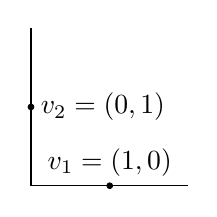
\begin{tikzpicture}
		\draw[black, thin] (0, 0) -- (2, 0);
		\draw[black, thin] (0, 0) -- (0, 2);
		\filldraw[black] (1,0) circle (1pt) node[anchor=south] {$v_1 = (1, 0)$};
		\filldraw[black] (0,1) circle (1pt) node[anchor=west] {$v_2 = (0, 1)$};
	\end{tikzpicture}
    \caption{Four cones for $N$ with rank $2$.}
    \label{fig:example-cones}
    \end{figure}

    In the Figure \ref{fig:example-cones}, the four cones spanned by the sets $\{(0, 1), (1, 0)\}$ are: $\{(0, 0)\}; \{(1, 0)\}; \{(0, 1)\}; \{(1, 0), (0, 1)\}$. 

    Cones constitute fans if certain conditions on the faces hold on these cones and thus give the definition of a fan:
    \begin{definition}
        A collection $\Sigma$ of strongly convex rational polyhedral cones in $N \R$ is called a \emph{fan} if 
	    \begin{enumerate}
		\item[(1)] each face of a cone in $\Sigma$ is also a cone in $\Sigma$, and 
		\item[(2)] the intersection of two cones in $\Sigma$ is a face of each. 
    	\end{enumerate}
    \end{definition}
    This means that all the cones in a fan are closed under intersection and taking faces. 

%% Subsection 
\subsection{Connection between toric varieties and fans}
\label{subsec:toric-variety-fan}
    Toric varieties and fans are tightly connected in the sense
    that we can construct a toric variety from a fan structure and vice versa. 
    Let us find the fan from a simple toric variety $\C\P^2$.
    In order to find a fan -- a collection of cones that live in $N_{\R}$, we start from the lattice itself $N$.
    It is known that there exists a one-to-one correspondence between cones in a fan and $T$-invariant subvarieties 
    as closures of $T$-orbits. 
    Although the details of this proof is not provided here, 
    we exploit this fact and start from finding the $T$-invariant subvarieties.
    Then we try to can find the corresponding cones for each $T$-invariant subvariety.

    Let $T$ be the torus $\{(1, t_1, t_2) | t_i \in \C^\ast\} \simeq (\C^\ast)^2 \subset \C\P^2$.
    Consider the lattice $N = \hom(\C^\ast, T)$ 
    such that elements of $N$ are homomorphisms $\psi: \C^\ast \rightarrow T$,
    which are called one-parameter subgroups, with the only parameter $t$. 
    We claim that the lattice $N = \hom(\C^\ast, T) \cong \Z^2$ 
    by the map $\phi: \Z^2 \mapsto N$ defined as follows:
    \[
    \phi(a, b) \mapsto (t \mapsto (t^a, t^b))
    \] 
    where $(a, b) \in \Z^2, t \in \C^\ast$.

    Let $f$ be the induced inclusion map $f: \C^\ast \rightarrow \C\P^2$ defined as $f(t) = \psi(t) \cdot 1_{\C\P^2}$. 
    Note that image of $f$ is still entirely contained in $T$.
    We want to find sets that are $T$-invariant, or invariant under action by $T$. 
    From group theory, we know that these are called $T$-orbits.
    Taking the closures of $T$-orbit on images of $f$ as $t \rightarrow 0$, 
    we obtain $T$-invariant 
    \[Z_\psi = \overline{T \cdot \lim_{t \rightarrow 0} f(t)}.\]

%% Subsection 
\subsection{Example of constructing a toric variety from a fan}
\label{subsec:contructing-toric-variety}
    Let us see an example by taking a lattice point $(a, b) = (0, 1)$.
    For any $x \in \C^\ast$, $\psi(x)= (x^0, x^1) = (1, x) \in T$. Then $f(x) = (1, 1, x) \in \C\P^2$. 
    Then $\lim_{x \rightarrow 0} f(x) = (1, 1, 0) \in \C\P^2$.
    The orbit of $T$ acting on $\lim_{t \rightarrow 0} f(x)$ is $\{(t_1, t_2) \cdot (1, 1, 0)\} = \{(1, t_1, 0)\} \in \C\P^2$
    where $(t_1, t_2) \in T$.
    Thus, we obtain the line $\{t_2 = 0\}$. 

    We can see from the above example that the relationship amongst $a, b, 0, 1$ are determinant of the cone,
    and these relationships divide the space into different areas,
    each corresponds with a cone. 
    We can then glue all the cones together to find fan. 

    \section{Toric Variety of Projective Spaces}
\label{sec:toric-variety-of-projective-spaces}
    We see in Section \ref{sec:tropical-arithmetic-valuations-tropical-plane-curves} that tropical varieties induce interesting combinatorial objects and polyhedral complexes give us tools for viewing old problems in new ways.
    We now introduce \textbf{polytopes}
    more formally and actually connect fans and their associated toric varieties with polytopes.
    In this section we follow the treatment and examples of \citet{Fulton1993} and \citet{Ranganathan2012}
    
    Roughly put, given a polytope, 
    we can define a fan whose rays are normal to the facets of the polytope that is determined by the toric variety associated with the fan.
    Here we don't give explicit constructions of these polytope but only show these polytopes and their associated projective spaces, to help the readers gain some geometric intuition.

        The polytope of $\P^3$, 
        which we have shown is a toric variety, 
        is the tetrahedron. 
        
        \begin{figure}
        \label{fig:tetrahedron}
        \begin{center}
        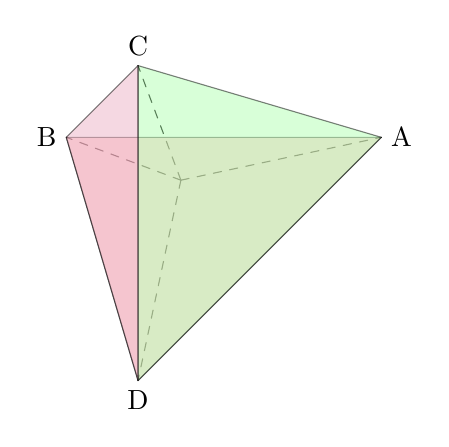
\begin{tikzpicture}[line join = round, line cap = round]
        \pgfmathsetmacro{\factor}{1/sqrt(2)};
        \coordinate [label=right:A] (A) at (2,0,-2*\factor);
        \coordinate [label=left:B] (B) at (-2,0,-2*\factor);
        \coordinate [label=above:C] (C) at (0,2,2*\factor);
        \coordinate [label=below:D] (D) at (0,-2,2*\factor);

        \foreach \i in {A,B,C,D}
        \draw[dashed] (0,0)--(\i);
        \draw[-, fill=red!30, opacity=.5] (A)--(D)--(B)--cycle;
        \draw[-, fill=green!30, opacity=.5] (A) --(D)--(C)--cycle;
        \draw[-, fill=purple!30, opacity=.5] (B)--(D)--(C)--cycle;
        \end{tikzpicture}
        \end{center}
        \caption{A tetrahedron, the polytope of $\P^3$}
        \end{figure}
        
        \begin{figure}
        \label{fig:fan-p2}
	    \begin{center}
	    \begin{tikzpicture}[axis/.style={thin, ->, >=stealth'}]
	    % Draw coordinates
		\draw[axis] (0, 0) -- (1, 0) node[right]{$v_1$};
		\draw[axis] (0, 0) -- (0, 1)
		node[above]{$v_2$};
		\draw[axis] (0, 0) -- (-1, -1) node[below]{$v_3$};
	    \end{tikzpicture}
	    \end{center}
	    \caption{The fan of $\P^2$.}
        \end{figure}
        
        \begin{figure}
        \begin{center}
        \begin{tikzpicture}
        \label{fig:polytope-p2}
        \draw (-2,0) node[anchor=north]{$A$}
        -- (2,0) node[anchor=north]{$C$}
        -- (0,4) node[anchor=south]{$B$}
        -- cycle;
        \end{tikzpicture}
        \end{center}
        \caption{The polytope of $\P^2$}
        \end{figure}
        
        \begin{figure}
        \label{fig:fan-p1-p1}
	    \begin{center}
	    \begin{tikzpicture}[axis/.style={thin, ->, >=stealth'}]
	    % Draw coordinates
		\draw[axis] (0, 0) -- (1, 0) node[right]{$v_1$};
		\draw[axis] (0, 0) -- (0, 1)
		node[above]{$v_2$};
		\draw[axis] (0, 0) -- (-1, 0) node[below]{$v_3$};
		\draw[axis] (0, 0) -- (0, -1) node[below]{$v_4$};
	    \end{tikzpicture}
	    \end{center}
	    \caption{The fan of $\P^1 \times \P^1$.}
        \end{figure}
        
        \begin{figure}
        \label{fig:polytope-p1-p1}
        \begin{center}
        \begin{tikzpicture}
        \draw (1,1) node[anchor=south]{$A$}
        -- (-1,1) node[anchor=south]{$B$}
        -- (-1,-1) node[anchor=north]{$C$}
        -- (1,-1) node[anchor=north]{$D$}
        -- cycle;
        \end{tikzpicture}
        \end{center}
        \caption{The polytope of $\P^1 \times \P^1$}
        \end{figure}
    
        \begin{figure}
        \label{fig:polytope-p1-p1-p1}
        \begin{center}
        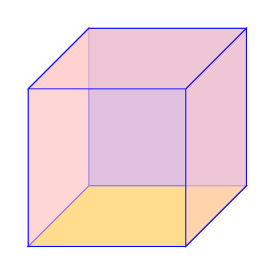
\begin{tikzpicture}
        \coordinate (O) at (0,0,0);
        \coordinate (A) at (0,\Width,0);
        \coordinate (B) at (0,\Width,\Height);
        \coordinate (C) at (0,0,\Height);
        \coordinate (D) at (\Depth,0,0);
        \coordinate (E) at (\Depth,\Width,0);
        \coordinate (F) at (\Depth,\Width,\Height);
        \coordinate (G) at (\Depth,0,\Height);

        \draw[blue,fill=yellow!80] (O) -- (C) -- (G) -- (D) -- cycle;% Bottom Face
        \draw[blue,fill=blue!30] (O) -- (A) -- (E) -- (D) -- cycle;% Back Face
        \draw[blue,fill=red!10] (O) -- (A) -- (B) -- (C) -- cycle;% Left Face
        \draw[blue,fill=red!20,opacity=0.8] (D) -- (E) -- (F) -- (G) -- cycle;% Right Face
        \draw[blue,fill=red!20,opacity=0.6] (C) -- (B) -- (F) -- (G) -- cycle;% Front Face
        \draw[blue,fill=red!20,opacity=0.8] (A) -- (B) -- (F) -- (E) -- cycle;% Top Face
        \end{tikzpicture}
        \end{center}
        \caption{The polytope of $\P^1 \times \P^1 \times \P^1$}
        \end{figure}
    
    
%%% Chapter 3: Intersection Theory
\chapter{Intersection Theory}
\label{chp:intersection-theory}

\epigraph{
From time to time you rub so the liquid penetrates better, and otherwise you let time pass. The shell becomes more flexible through weeks and months -- when the time is ripe, hand pressure is enough, the shell opens like a perfectly ripened avocado!
}{Alexander Grothendick}

Intersection Theory stands in the center of algebraic geometry. 
It gives information about the intersection of subvarieties of a given variety. 
A very baby manifestation of the spirit of intersection theory is 
B\'{e}zout's Theorem

	\begin{theorem}[B\'{e}zout's Theorem]
		If two plane curves $A, B \subset \P^2$ intersect, 
		then they intersect at $(\deg A)(\deg B)$ points. 
	\end{theorem}
	
Another manifestation of intersection theory is Gauss' fundamental theorem of algebra:
	\begin{theorem}[Fundamental Theorem of Algebra]
		A non-zero, single-variable, 
		degree-$n$ polynomial with complex coefficients has, 
		counted with multiplicity, exactly 
		$n$ complex roots.
	\end{theorem}
We will introduce the notion of \emph{Chow ring} 
and its connection associated with homology and cohomology. 
Before we formally start and to give some flavor,
\textbf{Chow groups} are abelian groups associated to a geometric object
that are described as a group of cycles modulo an equivalence relation.
When the variety is smooth, 
the intersection product makes the Chow groups into a graded ring,
the Chow ring.
This Chow ring structure is parallel to the ring structure 
on the homology of a smooth compact manifold
that can be imported using Poincar\'{e} duality
from the natural ring structure on cohomology. 
Later we will see that 
the cohomology ring coincides in some cases with the Chow ring which facilitates our calculation of the cohomology ring. 

For readers who are unsatisfied with our very brief treatment of 
such a rich theory, 
we recommend the classic textbook \emph{Intersection Theory} 
by \citet{Fulton1998} for additional details.
Another textbook that treats this subject starting from an elementary level
is \emph{3264 and All That: A Second Course in Algebraic Geometry} by \citet{Eisenbud2016} and we are following their treatment in this manuscript as well. 



	







	












    %%%% Section 2
\section{Cycles, Rational Equivalence and the Chow Group}
\label{sec:cycles-rational-equivalence-chow-group}
We want to define our most basic algebraic structure here.
	\begin{definition}[Free Abelian Group]
		A group $G$ is a \textbf{free abelian group}
		if 
		\[
		G \cong \bigoplus\limits_{i \in I} \Z
		\]
		for some arbitrary index set $I$. 
	\end{definition}
	A free abelian group has an associated basis $\calb$ if and only if
	$\calb$ generates $G$ and for $b_1, \ldots, b_n \in \calb$ 
	and $c_1, \ldots, c_n \in \Z$,  
	\[
	\sum\limits_{i=1}^n c_i b_i = 0,
	\]
	implies that $c_1 = \cdots = c_n = 0$. 
	

	\begin{definition}[Group of Cycles]
		Let $X$ be any algebraic variety. 
		The \emph{group of cycles} on $X$, denoted $Z(X)$,
		is the free abelian group generated by the set of subvarieties
		(or reduced irreducible subschemes) of $X$.
		
		The group $Z(X)$ is graded by dimension:
		we write $Z_k(X)$ for the group of cycles 
		that are formal linear combinations of 
		subvarieties of dimension $k$
		(these subvarieties are also called $k$-cycles),
		so that we have
		\[
		Z(X) = \bigoplus_k Z_k(X).
		\]
	\end{definition}

For subvarieties $Y_i \in X$ with some arbitrary index set $I$,
we call a cycle 
	\[
	Z = \sum\limits_{i \in I} n_i Y_i
	\] is \textbf{effective} if all the coefficients $n_i$ are nonnegative. 
In other words, a cycle on an arbitrary algebraic variety (or scheme) $X$
is a finite formal sum of (irreducible) subvarieties of $X$,
with integer coefficients.
For a given field $K$, we say that \textbf{rational functions}
are algebraic fractions with both numerators and denominators 
being polynomials.
U 

Another important definition that will appear many times in the future is 
	\begin{definition}[(Weil) Divisor]
		A \textbf{(Weil) divisor} is an $(n-1)$-cycle on a pure $n$-dimensional 
		scheme. 
	\end{definition}
How can we intuitively see divisor and why is it called divisor? 
Loosely speaking, divisors are integer linear combinations of 
codimension-$1$ subvarieties.
Let us think about an easy case ($1$-dimensioanl case): 
Given two plane curves and let them intersect,
the integer combination of the intersection points (possibly with multiplicity) 
is a divisor. 

	\begin{definition}[Rational Equivalence]
		We say that two $i$-cycles $Z_1$ and $Z_2$ 
		are rationally equivalent if and only if 
		there exists a subvariety $V \subset \P^1 \times X$ 
		and two points $x_1, x_2 \in \P$ such that
		\[
		(V \cap (\{x_1\} \times X)) - (V \cap (\{x_2\} \times X)) = 0.
		\]
		
		We say that two subschemes are rationally equivalent if 
		their associated cycles are rationally equivalent.
	\end{definition}

	\begin{definition}[Chow Group]
		Let $\rat(X)$ be the set of rational equivalence classes 
		of cycles of $X$.
		The \textbf{Chow Group} of $X$ is the quotient
		\[
		A(X) = Z(X)/\rat(X),
		\]
		or in other words,
		the \textbf{group of rational equivalence classes of cycles 
		on $X$}. 
		If $Y \in Z[X]$ is a cycle, we write $[Y] \in A(X)$ 
		for its equivalence class;
		if $Y$ is a subscheme, we write $[Y]$ 
		as the class of the cycle $\inner{Y}$ associated to $Y$. 
	\end{definition}

We mentioned previously that Chow groups are graded by dimension,
and let us restate the following.
	\begin{theorem}
		If $X$ is a scheme then the Chow group of $X$ 
		is graded by dimensions;
		that is 
		\[
		A(X) = \bigoplus A_k(X)
		\]
		where $A_k(X)$ is the group of rational equivalence classes of
		$k$-cycles. 
	\end{theorem}

If we see through what B\'{e}zout's Theorem says,
we see that for plane curve $A$ and $B$, they at most intersect at 
$(\deg A)(\deg B)$ points with multiplicity. 
This implies that when we count the subvarieties that lie at the intersection,
there should be some ``product structure" analogous to "cup product" 
of cohomology ring that give us some ring structure.

Let us state this general theorem.
	\begin{theorem}[Unique Product Structure on $A(X)$]
		If $X$ is a smooth quasi-projective variety,
		then there is a unique product structure on $A(X)$ 
		satisfying the condition:
		If two subvarieties $A, B$ of $X$ are generally transverse;
		that is, they meet transversely at a general point of each component of $C$ of $A \cap B$,
		then we have
		\[
		[A][B] = [A \cap B].
		\]
		This structure makes the subvariety $A(X)$ 
		\[
		A(X) = \bigoplus\limits_{c = 0}^{\dim X} A^c(X)
		\]
		into an associative, commutative ring, 
		graded by codimension, called the Chow ring of $X$. 
	\end{theorem}
	The products rational equivalent cycles are in fact 
	rationally equivalent as well (see \citet{Fulton1993}). 
    \section{Computing the Chow Ring}
\label{sec:computing-the-chow-ring}
To derive some techniques for computing the Chow ring,
we start with the idea of \textbf{affine stratification},
which will be a powerful tool in calculating the Chow groups 
for the projective spaces, Grassmannians and other rational varieties.
The idea is that given a variety (or a scheme) $X$ that admits a affine stratification,
we can decompose $X$ into union of affine spaces.
	\begin{definition}
		A scheme $X$ is \textbf{stratified} by a finite collection of 
		irreducible, locally closed subschemes $U_i$ 
		if $X$ is a disjoint union of the $U_i$ and,
		in addition,
		the closure of any $U_i$ is a union of $U_j$ 
		-- in other words, 
		if $\overline{U_i} \cap U_j \ne \varnothing$,
		then $U_j \subseteq \overline{U_i}$.
		
		The collection of such $U_i$ is called the \textbf{strata} 
		of the stratification. 
		The collections of such $\overline{U_i}$ is called 
		the \textbf{closed strata} of the stratification.	
	\end{definition}
In the same fashion, sometimes we call $U_i$ 
the open strata just to be clear. Now establish two more definitions based on stratification.
	\begin{definition}
	\label{def:stratification}
		We say that a stratification of $X$ with strata $U_i$ is
		an \textbf{affine stratification} 
		if each open stratum is isomorphic to 
		some affine $k$-space $\A^k$
		and we call it \textbf{quasi-affine} 
		if each $U_i$ is isomorphic to an open subset of some $\A^k$.
	\end{definition}

	\begin{example}[Strata of $\P$]
		The closed strata of $\P$ is just $\P$.
		However, the open strata of $\P$ is  
		$\P \backslash \P^{i - 1} \cong \A$
		(see Hartshorne for how affine spaces can be covered 
		by affine spaces).
	\end{example}
	
A generalization of the previous example is the following:
	\begin{example}[Strata of $\P^i$]
		The closed strata for $\P^i$ is still just $\P^i$,
		but the open strata are the affine spaces
		$U_i = \P^i \backslash \P^{i-1} \cong \A^i$. 
		Notice that this strata can be given by the 
		\textbf{flag} (a sequence of subspaces) 
		\[
		\P^0 \subset \P^1 \subset \cdots \subset \P^n.
		\]
	\end{example}

Now let us state a very important proposition
that will help us establish the techniques of using affine stratification 
to compute the Chow ring of a particular space
and make connections with the rational equivalence classes:
	\begin{proposition}
		If a scheme $X$ has a quasi-affine stratification,
		then $A(X)$ is generated by the classes of the closed strata.
	\end{proposition}
    \section{Chow Ring and Cohomology}
From previous chapter, 
we learned that cohomology of a variety (or scheme) $X$
gives algebraic information about the intersection of subvarieties in $X$.
From a category theoretical point of view,
the cohomology is a contravariant functor from the category of algebraic varieties (or schemes) to the category of graded rings. 
Here we have seen that Chow ring is the exact analogy of cohomology.
We know that the Chow group $A^k(X)$ is generated 
by all the subdivarieties in $X$ of dimension $k$ 
with the rational equivalence relations between the subvarieties.
In the case of cohomology, the equivalence is homological equivalence 
induced by the coboundary maps, as we discussed before. 

Furthermore, for nonsingular toric varieties that have structure of 
a smooth manifold in the analytic topology, 
the Chow ring coincides with the de Rham cohomology of the variety.
This condition is sufficient for us to eventually calculate the 
cohomology ring of the heavy/light Hassett spaces using Chow ring. 

In this manuscript, we use $A^\ast(X)$ for the Chow ring of $X$
(not to be confused with the Chow group of $X$, $A(X)$) 
and $H^\ast(X; \Z)$ for the cohomology of $X$ with integer coefficients. Since this notation overrides the dual notation,
we denote the dual of the Chow ring (the intersection ring) as $A_\ast(X)$ 
and denote the homology using $H_\ast(X; \Z)$.
Notice that our previous discussion in this section states that
the intersection ring coincides with the homology 
for nonsingular toric varieties that have structure of a smooth manifold
in the analytic topology:
\[
A_\ast(X) \cong H_\ast(X; \Z).
\]

\subsection{Chow ring of projective $n$ space via toric variety and its associated fan}
	In fact, since $\P^n$ can be seen as toric varieties,
	the Chow ring can be further computed using combinatorial structures
	provided by the associated fan of the embedded toric variety.
	
	\begin{theorem}
		For a nonsingular projective variety $X$ 
		and its associated fan $\Sigma$,
		$A^\ast(X) = \Z[D_1, \ldots, D_d]/I$,
		where the $I$ is the ideal generated by all the 
		\begin{enumerate}	
			\item[(1)]
			products of divisors whose associated primitive generators 
			do not form a cone in the fan;
			that is 
			\[
			D_{i_i} \times \cdots \times D_{i_k}
			\]
			where $v_{i_1}, \ldots, v_{i_k}$ do not form a cone 
			in the fan $\Sigma$. 
			
			\item[(2)]
			$\sum\limits_{i = 1}^{d} \inner{u, v_i} D_i$
			for all the basis element $u$ that spans 
			the whole ambient vector space. 
		\end{enumerate}
	\end{theorem}
	
Let us calculate some Chow ring in some familiar spaces to practice the notion we just learned. 
	\begin{example}[Chow ring of $\P^3$]
		Recall that the primitive generators are 
		\begin{align*}
		v_1 &= (-1, -1, -1), v_2 = (1, 0, 0) \\
		v_3 &= (0, 1, 0), v_4 = (0, 0, 1) \\
		\end{align*}
		and the maximal cones are spanned by the following 
		sets of primitive generators
		\begin{align*}
		S_1 = \{v_1, v_2, v_3\}, \\
		S_2 = \{v_1, v_2, v_4\}, \\
		S_3 = \{v_1, v_3, v_4\}, \\
		S_4 = \{v_2, v_3, v_4\}, \\
		\end{align*}
		since four of the primitive generators together 
		do not span any cone. 
		We can check that the lower dimensional cones 
		can be found by intersecting the higher dimensional cones,
		which satisfy the condition for a fan. 
		
		To construct calculate Chow ring, we following 
		the previous theorem to find the generators of the ideal.
		We know that they have two types:
		\begin{enumerate}
			\item[(1)] The first type is the product of 
				all the primitive generators that do not span a cone.
				Notice that the only set of generators that 
				do not span a cone is the set full set 
				$\{v_1, v_2, v_3, v_4\}$,
				which gives us 
				\[
				D_1 D_2 D_3 D_4 \in I.
				\]
			\item[(2)] 
				The ambient vector space can be seen as 
				spanned by $\calb = \{v_1, v_2, v_3\}$,
				and thus this is a basis.
				Now for each basis element $u \in \calb$,
				we set 
				\[
				\sum\limits_{i = 1}^{d} \inner{u, v_i} D_i = 0. 
				\] 
				Thus for the basis element $v_1$, we have
				\[
				\sum\limits_{i = 1}^d \inner{v_1, v_i} D_i 
				= 1 \cdot D_1 + 0 \cdot D_2 + 0 \cdot D_3 - 1 \cdot D_4 = D_1 - D_4 = 0,
				\] and thus $D_1 = D_4$. 
				For $v_2$, we have 
				\[
				\sum\limits_{i = 1}^d \inner{v_2, v_i} D_i 
				= 0 \cdot D_1 + 1 \cdot D_2 + 0 \cdot D_3 - 1 \cdot D_4 = D_1 - D_4 = 0,
				\] and thus $D_2 = D_4$. 
				For $v_3$, we have 
				\[
				\sum\limits_{i = 1}^d \inner{v_2, v_i} D_i 
				= 0 \cdot D_1 + 0 \cdot D_2 + 1 \cdot D_3 - 1 \cdot D_4 = D_3 - D_4 = 0,
				\] and thus $D_3 = D_4$. 
				Therefore, 
				we have obtained another equivalence relation 
				that we need to mod out 
				\[
				D_1 = D_4, D_2 = D_4, D_3 = D_4.
				\]
				The generator of the ideal 
				that we obtain from step (1)
				can be rewritten using this relation as 
				\[
				D_1 D_2 D_3 D_4 = D_4^4
				\]
				Since now the divisors are all the same,
				renaming $D_i = H$, 
				we obtain the Chow ring of $\P^3$
				\[
				A^\ast(X) = \Z[H]/\inner{H^4}
				\]
				which recovers the result from the theorem 
				in previous section 
				where the proof does not use the combinatorial 
				structure of the associated fan of the toric variety 
				but only the geometric information 
				of the intersection of the subvarieties. 	
		\end{enumerate}
	
	\end{example}	
	
	\begin{example}[Chow ring of $(\P^1)^3$]
		Recall that the primitive generators are 
		\begin{align*}
		v_1 &= (1, 0, 0), \\
		v_2 &= (-1, 0, 0), \\
		v_3 &= (0, 1, 0), \\
		v_4 &= (0, -1, 0), \\
		v_5 &= (0, 0, 1), \\
		v_6 &= (0, 0, -1),
		\end{align*}
		The maximal cones are again generated by 
		every three of those generators.
		But since there are linearly dependent generators,
		we can only form $8$ top-dimensional (dimension $3$) cones,
		spanned by the following spanning sets:
		\begin{align*}
		S_1 = \{v_1, v_3, v_5\}, \\
		S_2 = \{v_1, v_3, v_6\}, \\
		S_3 = \{v_1, v_4, v_5\}, \\
		S_4 = \{v_1, v_5, v_6\}, \\
		S_5 = \{v_2, v_3, v_5\}, \\
		S_6 = \{v_2, v_3, v_6\}, \\
		S_7 = \{v_3, v_4, v_5\}, \\
		S_8 = \{v_4, v_5, v_6\}, \\
		\end{align*}
		
		Readers might already realize that 
		generators that are opposite directions cannot generate 
		higher dimensional cones.
		Thus the following sets cannot generate non-trivial cones
		$\{D_1, D_2\}$, $\{D_3, D_4\}$, $\{D_5, D_6\}$
		and all the unions of the three sets. 
		Thus we have
		\[
		D_1D_2 = 0, D_3 D_4 = 0, D_5 D_6 = 0,
		\]
		for the first type relation that yield the generators of the ideal.
		Then since the ambient vector space is $3$-dimensional,
		we select a basis $\calb = \{v_1, v_3, v_5\}$
		and for each basis element we do the following:
		Now for each basis element $u \in \calb$,
		we set 
		\[
		\sum\limits_{i = 1}^{d} \inner{u, v_i} D_i = 0. 
		\] 

		 For the basis element $v_1$, we have
				\[
				\sum\limits_{i = 1}^d \inner{v_1, v_i} D_i 
				= D_1 -  D_2  = 0, 
				\] and thus $D_1 = D_2$. 
				For $v_3$, we have 
				\[
				\sum\limits_{i = 1}^d \inner{v_3, v_i} D_i 
				=  D_3 -  D_4  = 0, 
				\] and thus $D_3 = D_4$. 
				For $v_5$, we have 
				\[
				\sum\limits_{i = 1}^d \inner{v_2, v_i} D_i 
				= D_5 - D_6  = 0,
				\] and thus $D_5 = D_6$. 
		In summery, the relations we have is thus
		\[
		D_1^2 = D_3^2 = D_5^2 = 0.
		\]
		Thus writing $D_1 = X, D_3 = Y, D_3 = Z$,
		the Chow ring of $\P^3$ is thus $\Z[X, Y, Z]$.
	\end{example}
	
	We state the general formula for projective $n$-space. 
	\begin{theorem}
		The Chow ring of $\P^n$ is 
		\[
		A(\P^n) = \Z[\zeta]/(\zeta^{n+1})
		\],
		where we say that $\zeta \in A^1(\P^n)$ 
		is the rational equivalence class of a hyperplane;
		ore more generally, the class of a variety of codimension $k$ 
		and degree $d$ is $d \zeta^k$.
	\end{theorem}
    \input{intersection-theory/sec-derivation-of-chow-ring-of-projective-spaces}

%%% Chapter 4: Tropicalization
\chapter{Tropicalization}
\label{chp:tropicalization}
\epigraph{
Algebra is the offer made by the devil to the mathematician...All you need to do, is give me your soul: give up geometry
}{Michael Atiyah}

In this chapter,
we will explore one of the central topics in tropical geometry:
trees and their parameter spaces.
We first start from the study of linear spaces,
which set our journey to begin from the study of hyperplane arrangements.
These hyperplane arrangements push us to the combinatorial world,
where we incorporate the theory of matroids, 
borrowed from classical combinatorics and theoretical computer science.
We will see that the tropicalized linear spaces 
can be parameterized by the Grassmannian;
in particular, the Grassmannian $\gr(2, n)$
parameterizes the lines in the projective space $\P^{n-1}$,
and the tropicalization of it 
can be ``identified" with the space of phylogenetic trees 
from computational biology. 
All these set the foundations for us to study the tropicalization of 
a complete intersection, 
which is the subject of intersection theory in later chapter.

We first review some basic constructions in polyhedral geometry in section 1.
Tropical geometry has a strong connection 
with polyhedral geometry,
mostly because the tropical varieties will give us polytope, 
which gives us rich combinatorial structures. 
Polyhedral fans are tightly connected with toric varieties,
which in later chapters will be an important tool for
solving classical algebraic geometry problems. 
In this chapter, we are mainly following the treatment of \citet{Maclagan2015} and various articles cited inline. 



	
	
	
	
	
	
	
		


	

  


    \section{Convexity, Polyhedral Complices and Regular Triangulations} 
\label{sec:convexity-polyhedral-complices-and-regular-triangulations}

	\begin{definition}[Convexity]
		A set $X \subseteq \R^n$ is \textbf{convex} if,
		for all $\mathbf{u}, \mathbf{v} \in X$
		and all $0 \le \lambda \le 1$,
		we have $\lambda \mathbf{u} + (1 - \lambda)\mathbf{v} \in X$.
		The \emph{convex hull} $\conv(U)$ of a set  
		$U \subseteq \R^n$ si the smallest convex set containing $U$.
		 If $U = \{\mathbf{u}, \ldots, \mathbf{u}_r\}$ is finite,
		 then 
		 \[
		 \conv(U) = \{\sum\limits_{i = 1}^r \lambda_i \mathbf{u}_i: 0 \le \lambda \le 1, \sum\limits_{i = 1}^{r} \lambda_i = 1\}
		 \]
		 is called a polytope. 
	\end{definition}
	
	\begin{definition}[Polyhedral Cone]
		A \textbf{polyhedral cone} is a non-negative hull of 
		finite subset of $\R^n$:
		\[
		C = \{\sum\limits_{i = 1}^r \lambda_i \mathbf{v}_i: \lambda_i \ge 0\}.
		\]
	\end{definition}
	
	\begin{definition}[Face of A Cone]
		A \textbf{face} of a cone is determined by a linear functional 
		(a linear map from its vector space to its field of scalar,
		which in this case is $\R$)
		$w \in \R^n$, via 
		$f_w(C) = \{\mathbf{x} \in C: w \cdot x \le w \cdot y, y \in C \}$.
	\end{definition}
	
	\begin{definition}[Polyhedral Fan]
		A \textbf{polyhedral fan} is a collection of polyhedral cones,
		the intersection of any two of which is a face of each.
	\end{definition}
	
	\begin{definition}
	    We say that a fan is \textbf{simplicial} 
	    if the generators of each cone are linearly independent over $\R$.
	\end{definition}
	
	\begin{remark}
	We have another description of convex set: 
	they are intersections of half spaces in $\R^n$.
	We can also say that polyhedron $P \subset \R^n$ 
	is the intersection of finitely many closed half spaces,
	which can be written as 
	\[
	P = \{x \in \R^n: Ax \le b \}
	\] 
	where $A \in \mathbf{M}_{d \times n}$ and $b \in \R^d$.
	We can view the polyhedron as the solution space 
	of a linear systems of inequalities. 
	\end{remark}
	
	\begin{definition}[Polyhedral Complex]
		A \textbf{polyhedral complex} is a collection $\Sigma$
		of polyhedra satisfying two conditions:
		if $P$ is in $\Sigma$, 
		then so is any face of $P$,
		and if $P$ and $Q$ lies in $\Sigma$ 
		then $P \cap Q$ is either empty or a face of both $P$ and $Q$.
	\end{definition}
	
	\begin{definition}[Cells of Polyhedral Complex]
		The polyhedra in a polyhedral complex $\Sigma$ 
		are called the \textbf{cells} of $\Sigma$. 
	\end{definition}
	
	\begin{definition}[Facets]
		Cells of $\Sigma$ that are not faces of any larger cell are
		\textbf{facets} of the complex.
	\end{definition}
	
	\begin{definition}[Support]
	\label{def:support-of-a-polyhedral-complex}
		The \textbf{support} $\supp(\Sigma)$ of a polyhedral complex 
		$\Sigma$ is the set 
		$\{\mathbf{x} \in \R^n: \mathbf{x} \in P, P \in \Sigma \}$.
	\end{definition}
	
	\begin{remark}
	It may seem like support is the same as a polyhedral complex. 
	However, there is a subtle difference:
	polyhedral complex is a collection or a set of polyhedra;
	support is the union of them. 
	In other words, 
	a polyhedral complex has an internal structure 
	in terms of what its constituent polyhedra are and 
	how they are arranged. 
	Taking the support ``forgets" the internal structure 
	and flattens it into an undifferentiated set of points.
	\end{remark}
	 
	\begin{definition}[Lineality Space]
	    Given a polyhedron $P$,
		the \textbf{lineality space} 
		of a polyhedron is the largest affine subspace 
		contained in $P$.
	\end{definition}
	Another way to put this linear space is:
	it is the largest linear subspace $V \subset R^n$ 
	with the property that if $x \in P, v \in V$,
	then $x + v \in P$ 
	(the vector $v$ functions as a linear transposition to $x$).
	
	The \textbf{affine span} of a polyhedron $P$ 
	is the smallest affine subspace containing $P$.
	The \textbf{dimension} of $P$ is 
	the dimension of the linear space along $P$.
	
	\begin{definition}[Pure]
		A polyhedral complex $\Sigma$ is \textbf{pure} 
		of dimension $d$ if every polyhedron in $\Sigma$ 
		that is not the face of any other polyhedron in $\Sigma$ 
		has dimension $d$. 
	\end{definition}
	
	The following definitions start to build up to 
	the connection between 
	tropical geometry and polyhedral geometry.
	
	\begin{definition}[Rational Polyhedron]
		Let $\Gamma$ be a subgroup of $(\R, +)$.
		A \textbf{$\Gamma$-rational polyhedron} 
		is 
		\[
		P = \{x \in \R^n: Ax \le b\},
		\]
		where $A$ is a $d \times n$ matrix with entries in $\Q$
		and $b \in \Gamma^d$. 
	\end{definition}
	
	\begin{definition}[Regular Subdivision]
		Let $v_1, \ldots, v_r$ be an ordered list of vectors 
		in $\R^{n+1}$ 
		and fix $w = (w_1, \ldots, w_r) \in \R^r$/
		The regular subdivision of $v_1, \ldots, v_r$ induced 
		by $w$ is the polyhedral fan with support
		$\pos(v_1, \ldots, v_r)$
		whose cones are $\pos(v_i: i \in \sigma)$,
		for all subsets $\sigma \subseteq [r]$
		such that there exists $\mathbf{c} \in \R^{n+1}$ 
		with $\mathbf{c} \cdot \mathbf{v}_i = w_i$ for $i \in \sigma$,
		and 
		$\mathbf{c} \cdot \mathbf{v}_i < w_i$ for $i \notin \sigma$.
	\end{definition}
	These regular subdivisions are the subdivision of the fan structure naturally induced by the tropical varieties, which we will see in the next section. 
	
	
    \section{Tropical Variety}
\label{sec:tropical-variety}
	Let $K[x_1^{\pm1}, \ldots, x_n^{\pm1}]$ 
	denote the ring of \textbf{Laurent polynomials} over $K$.
	Thus an arbitrary 
	Laurent polynomial $f \in K[x_1^{\pm1}, \ldots, x_n^{\pm1}]$ is 
	in the form 
	\[
	f = \sum\limits_{\mathbf{u} \in \Z^n} c_{\mathbf{u}}x^{\mathbf{u}}
	\]
	\begin{definition}[\citet{Maclagan2015}]
		Given a valuation,
		the \textbf{tropicalization} 
		\[
		\trop(f)(w) = \min\limits_{u \in \Z^n} (\val(c_\mathbf{u} + \sum\limits_{i = 1}^{n} u_i w_i)).
		\] 
		is a piecewise, linear, real-valued function
		$f: \R^{n+1} \rightarrow \R$ 
		that is obtained by replacing each coefficients $c_{\mathbf{u}}$ 
		by its valuation and 
		by performing all additions and multiplications 
		in the tropical semiring $(\R, \oplus, \odot)$.
	\end{definition}
	
	The variety of the Laurent polynomial $f \in K[x_1^{\pm 1}, \ldots, x_n^{\pm 1}]$ 
	is a hypersurface in the algebraic torus $T^n$ over the algebraically 
	closed field $K$:
	\[
	V(f) = \{ y \in T^n: f(y) = 0 \}.
	\]
	We can check that in fact $\trop(V(f)) = V(\trop(f))$.
	
	\begin{example}[A Tropical Line]
		We have seen this example in previous chapter.
		Let $f =  x + y + 42$. 
		Then $\trop(f) = \min(x, y, 0)$ since any constant is mapped 
		to $0$ under the canonical valuation.
		Thus we have 
		\[
		\trop(V(f)) = \{x = y \le 0\} \cup \{x = 0 \le y\} \cup \{y = 0 \le x \}.
		\]
		Since this tropical variety has degree of only $1$,
		we call it a \textbf{tropical line}, 
		shown in the next figure. 
		This result is consistent with our result from the tropical 
		plane curve section.
	\end{example}
	
	Now we make an important connection between 
	the polyhedral geometry of tropical hypersurfaces,
	and the tropical varieties. 
	\begin{proposition}
		Let $f \in K[x_1^{\pm 1}, \ldots, x_n^{\pm 1}]$ 
		be a Laurent polynomial.
		The tropical hypersurface $\trop(V(f))$ is the support of
		a pure $\Gamma_{\val}$-rational polyhedral complex 
		of dimension $n - 1 \in \R^n$.
		It is also the $(n -1)$-skeleton of the polyhedral complex 
		dual to a regular subdivision of the Newton polytope of 
		\[
		f = \sum c_\mathbf{u} x^\mathbf{u}
		\]
		given by the weights $\val(c_\mathbf{u})$ on the lattice points
		in the Newton polytope of $f$. 
	\end{proposition}
	This description of tropical varieties plays an important role in geometric tropicalization as we will see in later chapter. 

    \section{Hyperplane Arrangement} 
\label{sec:hyperplane-arrangement}
	Let $\cala = \{H_i: 0 \le i \le n\}$ 
	be an arrangement 
	(a finite set with some geometric configuration) of $n+1$ 
	hyperplanes in $\P^d$
	such that no hyperplanes intersect 
	with each other at infinitely many points up to translation.
	We are interested in how the complement $X = \P^d \setminus \cala$ 	is configured by these hyperplanes. 
	In fact, $X$ is a subvariety of the torus $T^n$,
	cut out by a linear system of equations.

	Let $\mathbf{b}_i \in K^{d+1}$ be the normal vector of 
	the hyperplane $H_i$;
	that is $H_i = \{\mathbf{z} \in \P^d: \mathbf{b} \cdot \mathbf{z} = 0\}$.
	Let $B \in \mathsf{M}_{(d+1)\times (n+1)}$ 
	with columns being $b_i$ 
	and $A \in \mathsf{M}_{(n-d)\times (n+1)}$ 
	with rows being the basis for the kernel of $B$.
	Let $I$ be the ideal in $K[x_0^{\pm 1}, \ldots, x_n^{\pm 1}]$ 
	generated by the linear forms 
	\[
	f_i = \sum\limits_{j = 0}^{n} a_{ij} x_j
	\] for $1 \le i \le n-d$.
	
	We embed $X$ into $T^n$ as a subvariety 
	as the following proposition.
	
		\begin{proposition}
			There is an isomorphism $\phi: X \rightarrow T^n$ 
			between 
			the arrangement complement $X = \P^d \setminus \cala$ 
			and the subvariety $V(I)$ of $T^n$,
			defined as 
			\[
			\mathbf{z} \mapsto (\mathbf{b}_0 \cdot \mathbf{z}:
			\cdots: \mathbf{b}_n \cdot \mathbf{z}).
			\]
		\end{proposition}
	First notice that our assumption about the hyperplane 
	makes them span the whole space.
	Also notice that the image of this isomorphism 
	is indeed contained in the torus $T^n$,
	since $\mathbf{z} \ne \mathbf{0}$
	and that the ideal is fixed by the diagonal action by $K^\ast$
	(so we mod out the $K^\ast$). 
	We leave it to the readers to check that 
	this map is an isomorphism.
	
	\begin{example}[Three Lines in $\P^2$]
		Let $\cala$ be the hyperplane arrangement in $\P^2$
		that consists of the following four lines 
		with corresponding normal vectors
		\begin{align*}
			H_0 &= \{x_1 = x_2\}, \mathbf{b}_0 = \threevector{0}{1}{-1}, \\
			H_1 &= \{x_0 = x_2 \}, \mathbf{b}_1 = \threevector{1}{0}{-1},\\
			H_2 &= \{x_0 = x_1 \}, \mathbf{b}_1 = \threevector{1}{0}{-1}.
 		\end{align*}
		Thus we have a matrix $B \in \mathsf{M}_{3 \times 3}$:
		\[
		B = 
		\begin{bmatrix}
			0 &  1 & 0 \\
			1 & 0 & 0 \\
			-1 & -1 & -1 
		\end{bmatrix}
		\]
		and the matrix $A \in \mathsf{M}_{3 \times 3}$ 
		can be chosen to be:
		\[
		A = 
		\begin{bmatrix}
			1 &  0 & -1 \\
			0 & 1 & 1 \\
			1 & -1 & 0 
		\end{bmatrix}.
		\]
		Thus the ideal defined by $A$ is thus 
		\[
		I = \inner{x_1 - x_3, x_2 + x_3, x_1 - x_2} \subset k[x_1^{\pm 1}, \ldots, x_5^{\pm 1}].
		\]
		This linear ideal defines a plane in $\P^4$ 
		and $V(I)$ is the intersection of that plane with torus $T^4$.
		The previous proposition identifies the linear variety $V(I)$ 
		with the complement $\P^2\setminus \cala$ 
		of our arrangement of three lines in the plane. 
	\end{example}
	
	In fact any ideal generated by linear forms 
	corresponds to some hyperplane arrangement;
	even if the linear forms are not homogeneous, 
	we can homogenize it. 
	
	To illustrates the connection between hyperplane arrangements
	and matroid theory,
	we introduce the following definitions
	\begin{definition}[Support]
		The \textbf{support} of a linear form 
		$l = \sum a_i x_i \in I$ is 
		$\supp(l) = \{i : a_i \ne 0\}$.
	\end{definition}
	
	\begin{definition}[Circuit]
	\label{def:circuit}
		A non-empty subset $C$ in $[n]$ is a circuit of $I$ 
		if $C = \supp(l)$ for some non-zero linear form $l$ 
		in the ideal $I$
		and $C$ is inclusion-free.
	\end{definition}
	
	\begin{remark}
		The inclusion-free requirement makes a circuit $C$ 
		a maximal independent subset of the linear forms
		since it must be reduced to the set 
		such that $C$ does not contain or be contained 
		in some other circuit. 
		This implies that a circuit in $I$ is also 
		a minimal linear dependence 
		of the columns of $B$, the $\mathbf{b}_i$'s. 
		
		
		With this property, 
		we point out that the set of linear forms $l_C$ in $I$ 
		is the union of all reduced Gr\"{o}bner bases for $I \cap K[x_0, \ldots, x_n]$.
		Also each circuit is one-to-one correspond to a linear form 
		in $I$. 
		The ideal also has at most $\binom{n+1}{d+2}$ circuits, 
	 	which is attained when all the minors of $B$ are non-zero. 
		This implies that when computing Gr\"{o}bner bases,
		the problem is essentially reduced to 
		a Gaussian elimination problem. 
	\end{remark}
	
	Let $I \subset K[x_0^{\pm 1}, \ldots, x_n^{\pm 1}]$ 
	be generated by linear forms,
	where $K$ has the trivial valuation,
	and consider the hyperplane arrangement complement 
	that is identified with the variety of an ideal of linear forms, 
	$X \cong V(I)$.
	We restate the above remark in our tropical language
	
	\begin{proposition}
		The set of linear polynomials $l_C$ in $I$
		whose supports are circuits is a tropical basis for $I$.
	\end{proposition}
	
	To see more geometric intuition, we state another version of 
	this proposition.
	\begin{proposition}
		A vector $\mathbf{w} \in \R^{n+1}/\R$ lies in $\trop(X)$ 
		if and only if, for any circuit $C$ of the ideal $I$,
		the minimum of the coordinates $w_i$ is attained at least twice,
		as $i$ ranges over all circuits in $C$.
	\end{proposition}
	
	\begin{example}[Homogenizing Ideals of Linear Forms]
		Consider the ideal 
		\[
		I' = \inner{1 + x_1 + x_2, x_1 + 42x_2 + 47 x_3}
		\subseteq K[x_1^{\pm 1}, \ldots, x_3^{\pm 1}]
		\]
		which defines a two dimensional subvariety $X$ 
		of $T^3$ because we have two linear forms
		with three coordinates.
		Homogenizing the ideal $I'$,
		we obtain 
		\[
		I = \inner{x_0 + x_1 + x_2 + x_3, x_1 + 42x_2 + 47 x_3}
		\subseteq K[x_0^{\pm 1}, \ldots, x_3^{\pm 1}].
		\]
		Thus the variety $X = V(I)$ is the complement of 
		some hyperplane arrangement of $4$ lines in the projective plane $\P^2$. 
	\end{example}
	
	\begin{example}[A Tropical Basis]
		Let $I$ be the homogenized ideal in the previous example:
		\[
		I = \inner{x_0 + x_1 + x_2 + x_3, x_1 + 42x_2 + 47 x_3}
		\subseteq K[x_0^{\pm 1}, \ldots, x_3^{\pm 1}].
		\]
		The set of circuits is 
		\[
		C_1 = \{0, 1, 2, 3\}, C_2 = \{1, 2, 3\}
		\]
		but it is not inclusion-free at this moment;
		we reduce it to the set of circuits
		\begin{align*}
			C_1 &= \{1, 2, 3\} \\
			C_2 &= \{0, 1, 2\} \\
			C_3 &= \{0, 1, 3\} \\
			C_4 &= \{0, 2, 3\}.
		\end{align*}
		By ranging over all this set of circuits and attaining minimum twice, we can obtain the tropical basis. 
	\end{example}

	We call such $\trop(X)$, a \textbf{tropicalized linear variety}.
	Later we will clarify the difference between 
	tropical linear variety and tropicalized linear variety. 
	The notion of circuits give us a combinatorial description 
	of the tropicalization of $\trop(X)$ 
	for a linear vareity $X$
	using teh the Gr\"{o}bner basis.
	To organize all the information embedded in the circuits
	-- their representation of minimal linear dependence 
	among all the column vectors $\mathbf{b}_i \in K^{d+1}$ 
	of the matrix $B$.
	
	\begin{definition}[Lattice of Flats]
	\label{def:lattice-of-flats}
		Given a linear variety $X$, 
		\textbf{lattice of flats} $\call(B)$ 
		the set of subspaces (flats) of $K^{d+1}$ 
		that are spanned by subsets of the column vectors of $B$.
	\end{definition}
	
	Organizing the lattice of flats into a poset $\call(B)$ of rank $d+1$
	according to subspace relations with abuse of notation,
	we obtained a \textbf{simplicial complex},
	set composed of points, line segments, triangles, 
	and their $n$-dimensional counterparts,
	and we call it \textbf{order complex} of the poset.
	

    \section{Regular Triangulations}
\label{sec:regular-trangulations}
    We will not dive into the details of triangulations in this manuscript; however, it helps us formally visualize the polyhedral complices induced by tropical varieties. 
	\begin{definition}[Triangulation]
		A \emph{triang
		ulation} $T$ of a point set 
		$\cala = \{a_1,\cdots,a_n\}$ is a set of simplexes 
		such that their vertices are in $\cala$, 
		their union equals the convex hull $\conv(A)$, 
		and the intersection of any pair of simplexes 
		is their common (possibly empty) face.
	\end{definition}
	
	For a fixed triangulation $T$ of $\cala$,
	every vector $\phi \in \R^n$ induces a unique piecewise linear 
	function $g_{\phi, T}(a_i) = \phi_i$ 
	at the vertices of $T$
	and by the requirement that 
	$g_{\phi, T}(a_i)$ should be an affine function 
	(meaning a linear function plus some constant
	such that it looks like a straight line in a plane
	or just linear space translated in higher dimensions)
	on each simplex of $T$.
	
	Now we give a slightly less technical definition of the regular 
	triangulations.
	\begin{definition}[Regular Triangulations]
		A triangulation $T$ of $\cala$ is said to be \textbf{regular}
		if there exists a vector $\phi \in \R^n$ 
		such that $g_{\phi, T}$ is strictly convex over $T$.
	\end{definition}
	
	From this definition,
	we can already see how these polyhedral complices are 
	connected to tropical geometry
	via this simple relationship between 
	the regular triangulation in $\R^d$ 
	and the convex hulls in $\R^{d+1}$.
	By having this piecewise linear function 
	$\phi: \cala \rightarrow \R$,
	we are simply lifting every point $a_i \in \cala$ 
	to the graph of $\phi$,
	which form a convex hull above the graph formed by 
	all the vertices in $\cala$. 
	The \emph{lowest} part of this convex hull 
	is thus the graph of the convex piecewise linear function.
    \section{Geometric Tropicalization}
\label{sec:geometric-tropicalization}
    Given a subvariety (or subscheme) $X \subset T^n$ embedded in a torus,
    we can see that the tropical variety $X^{\trop}$ in fact gives a good compactification of $X$
    using a technique called \textbf{geometric tropicalization}.
    Geometric tropicalization was first used to study compactification of subvarieties in \citet{Tevelev2007} and compactifications of moduli spaces of del Pezzo surfaces in \citet{Hacking2007}. References in this section are 
    \citet{Maclagan2015}, \citet{Payne2014},
    \citet{Cavalieri2014}
    and 
    \citet{Cueto2011}.
    
    \begin{definition}[Boundary, Divisorial]
    \label{def:boundary-divisorial}
        Let $X$ be a very affine variety,
        and $\overline{X}$ is a compactification of $X$.
        We call the set $\partial \overline{X} = \overline{X}/X$
        the \textbf{boundary}.
        If the boundayr $\partial \overline{X}$ is a union of codimension-one subvarieties of $\overline{Y}$, 
        we say the boundary is \textbf{divisorial}.
    \end{definition}
    
    \begin{definition}[Combinatorial normal crossings divisor]
    \label{def:combinatorial-normal-crossings-divisor}
        Let $D_1, \ldots, D_l$
        be the irreducible components of $\partial \overline{X}$.
        The boundary $\partial \overline{X}$ is a \textbf{combinatorial normal crossings divisor}
        if, 
        for any subset $\sigma \subseteq \{1, \ldots, l\}$,
        the intersection $\cap_{i \in \sigma} D_i$ has codimension $|\sigma|$ in $\overline{X}$.
    \end{definition}
    
    \begin{definition}[Simple Normal Crossings]
    \label{def:simple-normal-crossings}
        Let $\partial \overline{Y}$ be a combinatorial normal crossings divisor.
        for any subset $\sigma \subseteq \{1, \ldots, l\}$,
        the intersection $\cap_{i \in \sigma} D_i$ is transverse,
        then the boundary is \textbf{simple normal crossings}.
    \end{definition}
    Here we say that if an intersection is \textbf{transverse}, then the intersection will have codimension equal to the sums of the codimensions of the two interesecting $D_i, D_j$.
    That is, transversality characterizes the most generic intersections.

    Given a variety (or a scheme) $X$
    with a simple normal crossing boundary divisor $D$,
    there exists a map $\psi$ from $X \setminus D$ to a torus $T$,
    such that this map is an embedding.
    The map induces a map from the dual intersection complex $\Sigma$ to the vector space of one paramter subgroupos of $T$, which we briefly discussed in Section \ref{sec:toric-variety},
    thus giving a fan structure on $\Sigma$. 
    
    Following the discussion of \citet{Cueto2011},
    we see that the top dimensional cones of $\Sigma$ associated with a weight function in fact produces a balanced fan.
    This fan gives a toric variety,
    allowing us to consider the closure of image of the map $\psi$.
    That is, we consider $\overline{\psi(X \setminus D}$ and its relationship with $X$. 
    
    Geometric tropicalization is an important techniques 
    that we will be use to understand the combinatorial structure of $\calm_{0, n}^{\trop}$ and the boundary stratification of $\overline{\calm}_{0, n}$ (see Definition \ref{def:stratification}).
    We will use geometric tropicalization to understand compactification of moduli spaces of smooth $n$-pointed curves and weighted curves in Section \ref{sec:geometric-tropicalization-for-m-0n}.
    For an interested reader, 
    we apologize for not diving into the details of tropical compactification, but we encourage readers to look into work \citet{Tevelev2004} and \citet{Maclagan2015}. 

    
    
    
    
    
    
    
    \section{Tropical Grassamanians}
\label{sec:tropical-grassmannians}
    We begin our exploration families of varieties by starting with one of the object that parametrizes subvarieties, the Grassmannians.
    The tropical Grassmannian arises from the ideal of quadratic Pl\"{u}cker relations 
    and it parametrizes the tropical linear spaces.  
    We will see that the lines in tropical projective space are trees, 
    and their tropical Grassmannian $\gr(2, n)$ is the sapce of the Speyer -Sturmfels phylogenetic tress that we will study in \citet{Billera2002},
    \citet{Speyer2004}. 
    
    Studying Grassmannians and Pl\"{u}cker's coordinates will first show us that
    under Pl\"{u}cker embedding, the Grassmannians are projective varieties,
    and further lead us to draw connections between the space of phylogenetic trees and moduli spaceso of curves. 
    References of this section are \citet{Maclagan2015}, 
    \citet{Speyer2003}, 
    \citet{Ranganathan2010},
    \citet{Hudec2007}
    
    
    First, we recall that the following definition.
    \begin{definition}[Tropical hypersurface]
    \label{def:tropical-hypersurface}
        Give a family of polynomials $F$ over an algebraically closed field $K$ with $n$ variables,
        the \textbf{tropical hypersurface} $T(F)$ of $F$ is the set of points in $\K^n$ such that the minimum is attained at least twice. 
        Equivalently, 
        $T(F)$ is the set of all points in $K^n$ where $F$ is not differentiable. 
    \end{definition}
    In the definition above, recall the Definition of tropical hypersurface in Section \ref{sec:convexity-polyhedral-complices-and-regular-triangulations}
    we mentioned that the tropical hypersurface is an $(n - 1)$-dimensional polyhedral complex in $K^n$. 
    
    %%%% Subsection
    \subsection{Grassmannians}
    \label{subsec:grassmannians}     
        \begin{definition}[Grassmannians]
        \label{def:grassmannians}
            Let $V$ be a vector space. 
            Grassmannian $\gr(r, V)$ is a space
            that parametrizes all the $r$-dimensional linear subspaces of the vector space $V$. 
            In another words 
            \[
            \gr(r, V) \coloneqq \{W \subset V: \dim W = r\}.
            \]
        \end{definition}
        
        \begin{example}[$\gr(2, 4)$]
        \label{ex:gr24}
            The set of all projective lines in the projective space $\P^3$ is $\gr(2, 4)$. 
        \end{example}
        
        An associative algebra defined on any vector space $V$ is called \textbf{exterior algebra}.
        The binary operation of any two element $v, w \in V$ is called \textbf{exterior product} or wedge product, denote as 
        \[
        v \wedge w
        \]
        such that $v \wedge w = - w \wedge v$. 
        \begin{example}
        \label{ex:v-wedge-v}
            For any $v \in V$, $v \wedge v = 0$.
            For any $v_i \in V$, 
            $i \in \lambda$ some arbitrary index set,
            $v_1 \wedge \cdots v_m = 0$ 
            whenever $v_i = v_{i + 1}$ for any $i \in \lambda$.
        \end{example}
        The wedge product of any two elements is called $2$-blade.
        Similarly,
        the wedge product of any $k$ elements is called
        $k$-blade. 
        
        \begin{definition}
        \label{def:exterior-power-of-a-vector-space}
            Let $V$ be a vector space.
            The $k$th exterior power of the vector space, denoted as $\bw^k V$ 
            is the span of all the $k$-blades of $V$.
            That is
            \[
            \bw^k V \coloneqq \vecspan{v_1 \wedge \cdots \wedge v_k: v_i \in V}. 
            \]
        \end{definition}
        
        \begin{definition}[Totally decomposible]
        \label{def:totally-decomposible}
            A element $w \in \bw^k V$ is said to be \textbf{totally decomposable}
            if it can be written as a $k$-blade;
            that is, if 
            \[
            w = w_1 \wedge \cdots \wedge w_k,
            \]
        \end{definition}
        
        \begin{example}[Non-example]
        \label{ex:not-totally-decomposable}
            The element $w = w_1 \wedge w_2 + w_3 \wedge w_4 \in \bw^k V$ is not totally decomposable. 
        \end{example}
        
        \begin{example}
        \label{ex:totally-decomposible-1}
            Every non-zero element of $\bw^1 V$ is totally decomposible. 
        \end{example}
        
        \begin{example}
        \label{ex:totally-decomposible-2}
            If $\dim V = 3$,
            then every non-zero element of $\bw^2 V$ is totally decomposable.
        \end{example}
        
        \begin{definition}[Divisor]
        \label{def:grassmannian-divisor}
            Let $w \in \bw^k V$,
            we say that $v \in V$ is a divisor of $w$ if there exists $u \in \bw^{k-1} V$ such that 
            \[
            w = v \wedge u. 
            \] 
        \end{definition}
        
        \begin{remark}
        \label{rem:space-of-divisors}
            One can see that if an element $w \in \bw^k V$ is totally decomposable,
            then the space of divisors is a subspace of dimension $k$ in $V$.
        \end{remark}
        
    %%%% Subsection
    \subsection{The Pl\"{u}cker Embedding of $\gr(r, V)$}
    \label{subsec:plucker-embedding-gr}
        \begin{lemma}
        \label{lem:plucker-embedding-lemma}
            Let $V$ be a vector space over some field $K$. 
            Let $W$ be a subspace of $V$ of finite dimension $r$ (i.e. $W$ is a point in $\gr(r, V)$).
            Let $\calb_1 = \vecspan{v_1, \ldots, v_r}$
            and $\calb_2 = \vecspan{w_1, \ldots, w_r}$.
            Then 
            \[
            v_1 \wedge \cdots \wedge v_r = \lambda(w_1 \wedge \cdots \wedge w_r)
            \]
            for some $\lambda \in K$. 
        \end{lemma}
        Note that $\lambda$ is the determinant of the change of basis matrix from $\calb_1$ to $\calb_2$.
        
        \begin{definition}[Pl\"{u}cker embedding]
        \label{def:plucker-embedding}
            A map $p: \gr(r, V) \rightarrow \P(\bw^r V)$ is defined as follows:
            given a subspace $W \in \gr(r, V)$ 
            and a basis $\calb_W = \vecspan{w_1, \ldots, w_r}$ of $W$,
            let $p: W \mapsto w_1 \wedge \cdots w_r$. 
            This map is the P\"{u}cker map
            and it embeds $\gr(r, V)$ into $\P(\bw^k V)$. 
        \end{definition}
        
        \begin{remark}
        \label{rem:plucker-embedding}
            Since different bases of $W$ will yield different multivectors of $\bw^r V$,
            but by Lemma \ref{lem:plucker-embedding-lemma},
            this map is unique up to scalar multiplication,
            hence a well-defined map on the \textbf{projectivization} of $\bw^r V$, 
            denoted as $\P(\bw^r V)$.
            We denote $p(W)$ as $[w]$.
            
            Notice that for any $v \in W$, 
            $p(W) \wedge v = 0 \in \bw^{k+1} V$.
        \end{remark}
        
        \begin{lemma}
        \label{lem:grassmannian-image-totally-decomposable}    
            $[w] \in \P(\bw^r V)$ 
            lies in the image of the Grassmannian 
            under the P\"{u}cker embedding 
            if and only if $w$ is totally decomposable.
        \end{lemma}
        The proof of this lemma is left to the readers.
        

        
        %%% Grassmannians as Projective Varieties
        \subsection{Grassmannians as projective varieties}
        \label{subsec:grassmannians-as-projective-varieties}
            We will use the Pl\"{u}cker embedding 
            and classify all the totally decomposable multivectors in $\bw^r V$ 
            as injections into the projective space $\P(\bw^r V)$. 
            
            \begin{theorem}[Injectivity of Pl\"{u}cker map]
            \label{thm:plucker-map-is-injective}
                The Pl\"{u}cker map is injective. 
            \end{theorem}
            
            \begin{proof}
                Define a map $\pi: \P(\bw^r V) \rightarrow \gr(r, V)$ as 
                \[
                \pi: [w] \mapsto \{v \in V| v \wedge w = 0 \in \bw^{r + 1} V\}.
                \]
                We want to show that $\pi \circ p = \id$;
                that is, $\pi \circ p(W) = W$ for any subspace $W \in \gr(r, V)$.
                Let $W \in \gr(r, V)$ with basis $\vecspan{w_1, \ldots, w_r}$.
                For any $w \in W$,
                $w \wedge [w_1 \wedge \cdots \wedge w_r] = 0$. 
                Thus $W \subseteq \pi \circ p(W)$.
                
                Let $v \in \pi \circ p(W)$, 
                then $v \wedge w_1 \wedge \cdots \wedge w_r = 0$,
                which implies $v$ is a linear combination of basis elements of $W$,
                and is thus in $W$. 
                
                Therefore, $W = \pi \circ p(W)$ 
                and $p$ is injective. 
            \end{proof}
            Such an injective map $p$ is indeed gives us the \textbf{Pl\"{u}cker embedding}.
            
            Now we identify the projectivization $\P(\bw^r V)$ with the projective space $\P^N$ as follows.
            For a basis $\calb_V = \vecspan{v_1, \ldots, v_n}$,
            we can choose $r$ basis elements to form a basis element of $\bw^r V$,
            each is linearly independent from others and the $\binom{n}{r}$ basis elements span the whole vector space $\bw^r V$ of dimension $\binom{n}{r}$.
            Projecting it, the projectivization $\P(\bw^r V)$ has dimension $N = \binom{n}{r} - 1$. 
            Thus we embed the Grassmannian $\gr(r, V)$ in $P(\bw^r V) = \P^n$ via the Pl\"{u}cker map. 
            That is 
            \[
            \gr(r, V) \subset \P^N, N = \binom{n}{r}.
            \]
            
            Now we define a similar map $\phi(w): V \rightarrow \bw^{d+1} V$ 
            for each $w \in \bw^r V$
            by $\phi_w(v) = w \wedge v$.
            Recalling Definition \ref{def:grassmannian-divisor}, 
            we notice that all the divisors of $w$ are in $\ker(\phi_w)$. 
            By Lemma \ref{lem:grassmannian-image-totally-decomposable}
            and Remark \ref{rem:space-of-divisors},
            we see that 
            \begin{corollary}
            \label{cor:rank-of-pi}
                For $w \in \bw^r V$, 
                $\phi_w$ has rank at most $n - r$.
                In particular, if $w$ is totally decomposable, $\phi_w$ has rank exactly $n-r$. 
            \end{corollary}
            
            Let us state the following theorem.
            \begin{theorem}
            \label{thm:grassmannian-is-projective-variety}
                The image of the Grassmannian is a projective variety.
                That is 
                \[
                p(\gr(r, V)) \subset P(\bw^r(V)).
                \]
            \end{theorem}
            This fact can be seen using the linear algebra fact that the rank of a matrix $M \in \mathsf{M}_{n\times m}(K)$ is the largest $r$ such that there exists non-zero $r \times r$ minors of $M$ and establishing a map $\psi: \bw^r(V) \rightarrow \hom(V, \bw^{d+1}(V))$ 
            such that $\psi(w) = \phi_w$.
            Using the maximality of the $(n - r) \times (n - r)$ minors, 
            a point $v \in \bw^r V$ lies in the locus of $(n - d + 1) \times (n - d + 1)$ minors of the matrix $\phi_w$, 
            which we view as a $n \times \binom{n}{d+1}$ matrix throughout this proof sketch.
            
            Another connection with linear algebra is the following.
            \begin{definition}[Pl\"{u}cker Coordinates]
            \label{def:plucker-coordinates}
                For a $r$-dimensional linear subspace $W \in \gr(r, V)$,
                the (homogeneous) coordinates of $p(W) \in \P^N$
                are the \textbf{Pl\"{u}cker coordinates} of $W$. 
            \end{definition}
            We remark that the coordinates are just 
            all the maximal non-vanishing minors of the matrix 
            whose rows are the basis of $W$. 
            
            \begin{example}
            \label{ex:plucker-coordinates-example-1}
                Consider the Pl\"{u}cker map of $\gr(1, n)$ maps a linear subspace $\vecspan{a_1 e_1 + \cdots + a_n e_n}$ is simply
                to the point $(a_1: \cdots : a_n) \in \P^{\binom{n}{1} - 1} = \P^{n-1}$. 
                Therefore, under this embedding, 
                $\gr(1, n) = \P^{n-1}$.  
            \end{example}
            
            \begin{example}
            \label{ex:plucker-coordinates-example-2}
                Consider the $2$-dimensional linear subspace 
                $W = \vecspan{e_1 + e_2, e_1 + e_3} \in \gr(2, 3)$.
                We can find its Pl\"{u}cker coordinates in $\P^{\binom{3}{2} - 1}$ in two ways.
                Take the wedge product of the basis elements, 
                $(e_1 + e_2) \wedge (e_1 + e_3) = 
                e_1 \wedge e_1 + e_2 \wedge e_1 + e_1 \wedge e_3 + e_2 \wedge e_3 = 0 - e_1 \wedge e_2 + e_1 \wedge e_3 + e_2 \wedge e_3$.
                Therefore, the coefficients this multivector is the Pl\"{u}cker coefficients of $W$ in $\P^2$;
                that is, $(-1, 1, 1)$. 
                
                Another way of seeing this is using the maximal minors othe matrix 
                \[
                M = 
                \begin{bmatrix}
                    1 & 1 & 0 \\
                    1 & 0 & 1 
                \end{bmatrix}
                \] where each row represents the coefficients of the canonical basis elements in the basis of $W$. 
                Calculating the maximal minors, we obtain the same answer $(-1, 1, 1)$.
                Notice that the any change of the spanning vectors only changes of the maximal minors by scalar multiplication,
                because the change is equivalanet to row operations on the matrix. 
                This example also confirms that the homogeneous Pl\"{u}cker coordinate of a point in $\gr(r, V)$ is well-defined. 
            \end{example}
            
            After working through Grassmannian and Pl\"{u}cker coordinates, 
            we will see how tropical Grassmannians are connected to phylogenetic trees in the next subsections. 
            
    \subsection{Space of Phylogenetic Trees}
    \label{subsec:grassmannians-and-space-of-phylogenetic-trees}
		A \textbf{phylogenetic tree} is tree $\tau$ 
		with finite labeled leaves
		and no vertices of degree two
		(because it must of degree three or above to avoid 
		bisecting an existing edge) 
		This is a notion arised from computational biology.
		We call the edges adjacent to the leaves of a phylogenetic 
		tree $\tau$ the \textbf{pendant edges} of $\tau$. 
		
		For any two leaves on a phylogenetic tree $\tau$,
		there exists a unique path 
		whose component edges have lengths.
		The sum of the lengths of all edges on a path between 
		leaves $i$ and $j$ is denoted  $d_{ij}$.
		The set of all distances, or metrics, on a tree $\tau$ 
		is called \textbf{tree metrics}
		and we thus obtain a metric space $[m]$. 
		
		For a tree $\tau$ with $n$ edges,
		we can put all the $\binom{n}{2}$ distances between 
		all pairs of $d_{ij}$ into a vector 
		$\mathbf{d} \in \R^{n \choose 2}$.
		Let $\Delta$ denote the set of all tree metrics in 
		$\R^{n \choose 2}$.
		The resultant metric space is called
		\textbf{space of phylogenetic trees}.
            
    %%% Subsection
    \subsection{Tropical Grassmannian and Tropical Linear Varieties from Phylogenetic Trees}
        In this subsection we study the tropicalization of Grassmannian
        and tropical linear varieties. 
        In particular, we will see how tropical linear spaces, 
        parametrized by Grassmannians, can correspond to phylogenetic trees.
        The recent work \citet{Dukkipati2013} proved that 
        there is a point on the tropical grassmannian that corresponds to each subtree of the phylogenetic tree.
        They also showed a necessary and sufficient condition for
        each of the subtree of a phylogenetic tree to be actually a fact of the tropical linear space. 
        The combinatorial structure of phylogenetic trees can reveal combinatorial structure of the tropicalization of the moduli spaces of curves. 
        
        The way we saw that $\gr(r, V)$ is a projective space in $\P^N$ 
        was through viewing $\gr(r, V)$ as the zero set of the maximal minors of a matrix. 
        Now we formally state that: 
        The Grassmannians are in fact the zero set of Pl\"{u}cker ideal,
        which is generated by all the Pl\"{u}cker relations.
        
        \begin{definition}
        \label{def:plucker-relation}
            For any two sequences $1 \le i_1 < \ldots < i_{r-1} < n$
            and $1 \le j_1 \le ldots \le j_{r+1} \le n$,
            the Pl\"{u}cker relation is defined as 
            \[
            \sum\limits_{m=1}^{r+1} (-1)^m p_{i_1, i_2, \ldots, i_{r-1}, j_m} p_{j_1, j_2,\ldots, \hat{j_a}, \ldots, j_{r+1}}
            \] where $\hat{j_a}$ means leaving out $j_a$ element.
        \end{definition}
        
        Let $I = \{i_l\}_{l=1}^{r-1}$, $J = \{j_k\}_{k=1}^{r+1}$.
        \begin{definition}[Pl\"{u}cker Ideal]
        \label{def:plucker-ideal}
            Let $I_{r, n}$ define the homogeneous ideal generated by all the Pl\"{u}cker relations, called \textbf{Pl\"{u}cker ideal}.
            That is,
            \[
            I_{r, n} = \inner{P_{I, J}: I, J \subseteq [n], |I| = r - 1, |J| = r + 1}
            \] where $P_{I, J}$ is the Pl\"{u}cker relations. 
        \end{definition}
        
        \begin{proposition}
        \label{prop:grassmannian-is-zero-setof-plucker-idea}
            The Grassmannian $\gr(r, V)$ is the subvariety of $\P^{\binom{n}{r} - 1}$ defined by this ideal.
        \end{proposition}
        
        \begin{definition}[Tropical Grassmannian]
        \label{def:tropical-grassmannian}
        The \textbf{tropical grassmannian} is $\trop(V(I_{r, n})$. 
        \end{definition}
        
        \begin{example}
        \label{ex:gr-24-plucker-ideal}
            For $\gr(2, 4)$, we can let $I = \{1\}, J = \{2, 3, 4\}$.
            \[
            P_{I, J} = -p_{12}p_{34} + p_{13}p_{24} - p_{14}p_{23}.
            \]
            Or equivalently, we could have $I = \{2\}, J = \{1, 3, 4\}$,
            or other $2$ possibilities, 
            which will give us the same relations up to sign.
            They all generate the same ideal, that is 
            \[
            I_{2, 4} = \inner{P_{\{1\}, \{234\}}} = \inner{P_{\{2\}, \{134\}}} = \inner{P_{\{3\}, \{124\}}} = \inner{P_{\{4\}, \{123\}}}.
            \]
        \end{example}
        
        \begin{example}
        \label{ex:gr-2n-plucker-ideal}
        In fact, the above example can be generalized to $\gr(2, n)$.
        We have
        \[
        I_{2, n} = \inner{p_{ij}p_{kl} - p_{ik}p_{jl} + p_{il} p_{jk}: i, j, k, l \in [n]}.
        \]
        The tropical Grassmannian 
        is thus $\trop(V(I_{2, n})) = \trop(V(p_{ij}p_{kl} - p_{ik}p_{jl} + p_{il} p_{jk}))$.
        Tropicalizing, we have that 
        \[
        \trop(V(I_{2, n})) = \{\text{the set of points where minimums of } p_{ij} + p_{kl},  p_{ik} + p_{jl},  p_{il} + p_{jk} \text{ is attained twice}\}
        \]
        \end{example}
        
        We state the following theorem from \citet{Dukkipati2013}.
        \begin{theorem}[Theorem 5.2, \citet{Dukkipati2013}]
            The Grassmannian $\gr(2, n)$ is equivalent to the space of all phylogenetic trees. 
        \end{theorem}
        For more detailed descriptions and study on the space of phylogenetic trees, we encourage readers to follow the refereces mentioned at the beginning of the section. 
        
        
        
        
        
        
            
            
            
            
            
            
            
            
            
            
        
        
        
        
        
        
        
        
        
        
        
        
        
        
        
    
    
    
    
    
    
    
    
    
    
    
    
    

%%% Chapter 5: Tropicalization of Spaces of Heavy/light weighted stable curve
\chapter{Cohomology of Hassett Spaces}
\label{chp:tropocalization-of-moduli-space-of-curves}
\epigraph{Geometry is the archetype of the beauty of the world.}{Johannes Kepler}
    We start with introducing basic concepts of moduli space.
    Hassett spaces are moduli spaces with weighted stable curves, 
    denoted as $\overline{\calm}_{g, w}$ for a particular genus $g$ and weight vector $w$.
    Then we base the work of \citet{Cavalieri2014}, 
    that showed that compactification and the fact 
    that it is a compactification of the hyperplane arrangements hold on these heavy/light Hassett spaces. 
    Then we want to find the tropicalization of the heavy/ligth Hassett spaces $\overline{\calm}_{0, w}$, 
    a polyhedral complex parametrizing leaf-labeled metric trees that can be thought of as Bergman fan, 
    which furthermore creates a toric variety $X_{\Sigma}$. 
    The work \citet{Cavalieri2014} showed that in the case when the weight vector $w$ is heavy/light, 
    the fan structure is isomorphic to $\calm_{0, w}^{\trop}$.
    However if the weights are not just heavy and light weights,
    we can still map $\overline{\calm}_{0, w}$ to the toric variety,
    by defining a natural projection $\pr_w$ associated with $w$,
    contracting some boundary strata.
    We will show that we can effectivize Theorem 6.7.14 in \cite{Maclagan2015}, 
    which states that there exists an isomorphism between the cohomology ring of the compactification of $\overline{\calm}_{0, w}$ 
    and the cohomology ring of the toric variety $X_\Sigma$.
    Hence, we could find the cohomology ring of $\overline{\calm}_{0, w}$
    by finding the the chow ring of $X_\Sigma$ which is can be calculated using the Bergman fan, 
    thereby giving a presentation of the intersection theory of these Hassett spaces.
    In this manuscript, 
    we follow the treatment of \citet{Cavalieri2014}
    and Chapter 6 of \citet{Maclagan2015}.




	



    \subsection{Moduli Space of Curves}
\label{sec:moduli-space-of-curves}
    Let us formally state the definition of a moduli space. 
    \begin{definition}[Moduli Space]
        A moduli space of algebraic curves is a geometric space 
        whose points represent isomorphism classes of algebraic curves.
    \end{definition}
    
    We proceed to give definition of Hassett spaces, moduli spaces of weighted stable curves.
    \begin{definition}
    \label{def:nodal-stable-curve}
    	A nodal, $n$-marked curve of genus $g$ is denoted as 
	    $(X, p_1, \ldots, p_n)$ 
	    where $p_i \in X(k)$ are the distinct nonsingular points of genus $g$
	    nodal curve $X$.
	    We say that a nodal, marked curve $(X, p_1, \ldots, p_2)$ 
	    is \textbf{stable} if the set of automorphisms 
	    \[
	    \aut(X, p_1, \ldots, p_n)
	    \]
	    is finite.
	    In other words, 
	    there are only finitely many automorphisms of the curve $X$ 
	    that fix each $p_1, \ldots, p_n$ pointwise. 
    \end{definition}
    
    For more advanced readers, 
    we can say that $(X, p_1, \ldots, p_n)$ is stable 
    if the restriction of $\omega_X(p_1 + \cdots + p_n)$ 
    to every irreducible component of $X$ is a line bundle of positive degree.
    Here $\omega_X$ is the dualizing sheaf of $X$.
    
    Given a weight vector, we have the following:
    \begin{definition}[Tropical $w$-stable curve]
    \label{def:tropical-w-stable-curve}
        Let $w = (w_1, w_2, \ldots, w_n) \in \Q^n$ 
        be a vector of weights satisfying $0 < w_i \le 1$ for all $i$ 
        and $\sum\limits_{i = 1}^{n} w_i > 2$.
        Let $C$ be a tree of $\P^1$'s, with $n$ smooth marked points 
        $p_1, p_2, \ldots, p_n$. 
        The curve $C$ is $w$-stable, if for each component $T$ of $C$,
        the sum 
        \[
        \sum\limits_{i;p_i \in T} w_i + \text{ number of nodes} > 2.
        \]
    \end{definition}
    If $w = (1^n)$, meaning all its entries are $1$'s,
    then $\overline{M_{0, w}} = \overline{M_{0, n}}$,
    which is the canonical moduli space of weighted stable curves. 
    
    We define heavy and light as follows 
    \begin{definition}[Heavy/light]
    \label{def:heavy-light}
    Let $w \in \Q^n$. Let $i \in [n]$.
    \begin{enumerate}
        \item $i$ is heavy in $w$, if for all $j \ne i$,
            we have $w_i + w_j > 1$. 
        \item $i$ is small in $w$, if $w_i + w_j > 1$ implies that $j$ is heavy in $w$. 
        \item if the total weights of small points is less than $1$,
        we say that they are light. 
    \end{enumerate}
    \end{definition}
    Usually we call weight vectors that contain only entries that are either heavy or light by \emph{heavy/light}. 
    Thus moduli spaces of heavy/light weighted stable curves are called Hassett spaces. 
    
    In \citet{Cavalieri2014}, we know for higher genus moduli spaces,
    they do not nicely embed into toric varieties. 
    However, for genus $0$, the compactification of $\calm_{0, w}$ can be obtained combinatorially. 
    We are interested in: for what weight vector $w$ can 
    the cone complex $\calm_{0, w}^{\trop}$ be given the structure of a balanced fan.
    They proved that 
    \begin{theorem}
    	The cone complex $\calm_{0, w}^{\trop}$ can be given the structure of a balanced fan 
	    in a vector space if and only if $w$ has only heavy and light entries. 
    \end{theorem} 
    
    \begin{theorem}
    	Let $w$ be a heavy/light weight vector.
	    There exists a toric variety $X_\Sigma$ with the torus $T_w$,
    	and an embedding of the Hassett space 
	    $\calm_{0, w} \hookrightarrow T_w$
	    such that 
	    \begin{enumerate}
		    \item[(1)] The         tropicalization of $\calm_{0, w}$ with respect to this embedding is 
			$\calm_{0, w}^{\trop}$.
		    
		    \item[(2)]
			The fan $\Sigma$ is $\calm_{0, w}^{\trop}$.
	    	
	    	\item[(3)]
			The closure of $\calm_{0, w}$ in $X_\Sigma$ is called 
			Hassett's compactification $\overline{\calm}_{0, w}$.
	\end{enumerate}
    \end{theorem}
    \section{Matroids}
\label{sec:matroids}
    In computer science theory and combinatorics, 
    there exists a mathematical generalization abstraction of the notion of independence 
    in vector space, which gives birth to matroid theory. 
    We can formalize a balanced fan in the language of matroid theory as follows, and introduce the definition of Bergmanfan in next section.
    \begin{theorem}[\citet{Cavalieri2014}]
    	The moduli space $\mathcal{M}_{0, w}^{\trop}$ with the heavy/light weights is the 
	    Bergman fan of a graphic matroid. 
    \end{theorem}
    
    Originated from computer science, a friendly definition of matroid is the following.
    \begin{definition}
        A finite matroid $M$ is a pair $(E, I)$, 
        where $E$ is a finite set called ground set,
        and $I$ is a set of subsets of $E$ (so called independent set)
        such that $I$ has the following properties:
    	\begin{enumerate}
		    \item[(1)]
			    The empty set is independent. Hence $I$ is not empty
		        and that any subset of an independent set is also independent. 
		        
		    \item[(2)]
			    For any $X, Y \in I$ such that $|X| > |Y|$,
			    there exists $e \in X$ such that $Y \cup \{e\} \in I$. 
	    \end{enumerate}
    \end{definition}
    
    %%% Graphic Matroid
    \subsection{Graphic Matroid}
    \label{subsec:graphic-matroid}
        In application, matroids can be used to generalize the notion of independence to graphs.
        Here is a concrete, classical example of a matroid called graphic matroid:
        Given any graph $G$ with the set of vertices $V$ and edges $E$.
        We define the matroid $M$ by letting the ground set $E(M)$ be the set of edges $E$
        and the independent set $I$ to be the set of all acyclic sets of edges. 
        
        Let us check that this pair $(E, I)$ satisfy the axioms of matroid:
        The set of edges is a finite set so we proceed to check independent set axioms.
        \begin{enumerate}
    	    \item[(1)]
		    The empty set $\varnothing \in I$ because it is certainly acyclic. 
		    Any subset of edges $Y$ of an acyclic set of edges $X$ certainly do not form any cycles;
		    since otherwise, the $X$ would have contained cycles to start with. 
	        
	        \item[(2)]
		    Let $X, Y \in I$ such that $|X| > |Y|$.
		    Assume for contradiction that adding any edge from $X$ to $Y$ 
		    will lead to an cyclic set of edges. 
		    This implies that the edges in $Y$ are incident to all the vertices 
		    connected by edges in $X$,
		    which furthermore implies that $|Y| \ge |X|$, a contradiction.
        \end{enumerate}
        Therefore, this $M = (E, I)$ is indeed a matroid, called ``graphic matroid".
	
	
	%%%% General Matroid
	\subsection{General Matroid}
	\label{subsec:general-matroid}
	    In our context, we use a generalization of the graphic matroid.
    	We abstract the ground set of the matroid to be 
	    $E = \{0, 1, \ldots, n\}$.
		\begin{definition}[Matroid]
			A \textbf{matroid} is a pair $M = (E, \calc)$ 
			where $E$ is the finite set and 
			$\calc$ is a collection of non-empty subsets of $E$,
			called the \emph{circuits} of $M$,
			that satisfies the following axioms:
				\begin{enumerate}
					\item[C1]
					    No proper subset of a circuit is a circuit.
					
					\item[C2]
						If $C_1, C_2$ are distinct circuits
						and $e \in C_1 \cap C_2$,
						then $(C_1 \cup C_2)\setminus \{e\}$
						contains a circuit.
				\end{enumerate}
		\end{definition}
		
		Additionally,
		we define flats of a matroid.
		\begin{definition}[Flat]
		\label{def:flat-of-a-matroid}
		    A \textbf{flat} of a matroid $M$ 
		    is the set $F$ such that $|C \setminus F| \ne 1$ 
		    for any circuit $C$. 
	    \end{definition}
	    
	    Recall the Definition \ref{def:circuit} of circuits.
	    We learned that the circuits of $X$ 
	    represents a tropical basis.
	    Thus we can associate a tropical linear space $\trop(X)$
	    with any given matroid $M$.
	
	\subsection{Connection with Tropical Linear Space}
	\label{subsec:tropical-linear-space}
	 
	    \begin{definition}
	    \label{def:tropical-linear-space}
	        Given a variety (or scheme) $X$, recall the definition of a tropical variety (see Section \ref{sec:tropical-variety})
	        The tropical variety $\trop(X)$ is a \textbf{tropical linear space}.
	    \end{definition}
	    In fact, we encountered this in our exposition of hyperplane arrangement (see Section \ref{sec:hyperplane-arrangement}),
	    where the open part of an variety $X$ that can be embedded in a torus is the complement of a $n+1$ hyperplane arrangement in a projective space. 
	    The compactifification of $X^{\trop}$ is a \textbf{wonderful compactification} of the hyperplane arrangement.
	    An interested reader can refer to work of \citet{Feichtner2005}.
	    In our case, the variety is exactly the moduli space of curves $\calm_{g, n}$,
	    and the Grassmannians (see Section \ref{sec:tropical-grassmannians}) parametrize their parameter spaces. 
	    The combinatorics of these tropical linear spaces can be studied using the theory of matroids. 


    \section{Bergman Fan and Nested Sets}
\label{sec:bergman-fan-and-nested-sets}
	We now describe a fan that is a generalization of 
	the simplicial fan generated from the lattice $\call(B)$ in Section \ref{sec:hyperplane-arrangement}.
	\begin{theorem}
		Let $M$ be a matroid on $E = [n]$.
		The collection of cones, 
		who is a positive span of the standard basis 
		associated with the all chains of flats of $M$,
		forms a pure simplicial fan of dimension $\rho(M) - 1$
		in $K^{n+1}/K$.
		The support of this fan equals the tropical linear space
		$\trop(M)$.	
	\end{theorem}
	The dimension of the simplicial fan can be explained as:
	since each chain of flats of the matroid $M$ can be extended to 
	a maximal chain, 
	and each maximal chain of flats $\rho(M) p- 1$ proper flats.
	
	In general, 
	$\trop(M)$ can be identified with $\Delta_M$, the order complex of 
	the geometric lattice of $M$.
	There is a coarser fan structure associated with $\trop(M)$ 
	give by the order complex as well, called \textbf{Bergman fan}.
	We describe the combinatorial description of this Bergman fan,
	since this aspect is the most concrete and computable aspect to us. 
	
    %% Subsection
    \subsection{Bergman Fan}
    \label{subsec:bergman-fan}
        \begin{definition}[Bergman Fan]
        \label{def:bergman-fan}
            For any matroid $M$ with ground set $E(M)$
            we associate a polyhedral fan, 
		    the Bergman fan $B(M) \subseteq \R^{|E|}$ 
		    in the following manner:
            \[
            B(M) \coloneqq \{w \in \R^{|E|}; M_w \text{is loop-free}\}
            \] 
            where $M_w$ is the matroid on $E$ 
            whose bases are all bases $B$ of $M$ of minimal 
		    $w$-weight $\sum_{i \in B}w_i$. 
        \end{definition} 

	    \begin{definition}[Equivalent definition of Bergman fan]
	    \label{def:bergman-fan-2}
    	    For a matroid $M$ on the ground set $[n] = \{1, 2, \ldots, n\}$,
    	    the Bergman fan $B(M) = \{w \in \mathbb{R}^n\}$ 
    	    such that for every circuit $C \in M$,
    	    the minimum of the set $\{w_i | i \in C\}$ is attained 
		    at least twice.
        \end{definition}
    
    %% Subsection
    \subsection{Nested Sets}
    \label{subsec:nested-sets}
        Work of \citet{Feichtner2005} and \citet{Maclagan2015},
        shows that there are several polyhedral structures constructed on the Bergman fan using the theory of building set.
        Recall that we introduced the definition of lattice of flats before (see Definition \ref{def:lattice-of-flats}
        and \ref{def:flat-of-a-matroid}).
        A building set is defined as 
        \begin{definition}[Definition 2.3, \citet{Cavalieri2014}]
        \label{def:building-set}
            Let $\calf$ be tha lattice of flats of a matroid $M$.
            For two flats $F, F' \in \calf$ we write $[F, F'] = \{G \in \calf: F \subseteq G \subseteq F'\}$. 
            A building set for $\calf$ is a subset $\calg$ of $\calf\setminus \{\varnothing\}$ such that the following holds:
            For any $F \in \calf\setminus \{\varnothing\}$, 
            let $\{G_1, \ldots, G_k\}$ be the maximal elements of $\calg$ contaiend in $F$.
            Then there is an isomorphism of partially ordered sets:
            \[
            \varphi_F: \prod\limits_{j=1}^{k} [\varnothing, G_j] \rightarrow [\varnothing, F],
            \] where the $j$-th component of $\varphi_F$ is the inclusion 
            $[\varnothing, F]$.
        \end{definition}
        
        \begin{definition}
        \label{def:nested-set}
            A subset $\cals$ of a building set $\calg$ is called \textbf{nested}, 
            if for any of incomparable elements $F_1, \ldots, F_l$ in $\cals$ with $l \ge 2$,
            the join of all the $F_i$ is not an element of $\calg$.
        \end{definition}
        \citet{Cavalieri2014} tells us that the nested sets of $\calg$ can form an abstract simplicial complex where a subset of a nested set is a nested set, coinciding with the definition of independent set of a matroid).
        By assigning each of the flat $F$ a vector $v_F \in \R^{[E]}$ 
        where $E$ is the ground set of the matrid,
        and accordingly a cone for each nested set of $\calg$,
        we obtain a polyhedral fan whose support (Definition \ref{def:support-of-a-polyhedral-complex}) is $B(M)$ where $M$ is the matroid. 
    
   	    \begin{definition}
    	\label{def:bergman-fan-quotient-space}
    	    Since for any matroid $M$,
    	    the Bergman fan contains the linear space $L$,
    	    spanned by the vector $(1, 1, \ldots, 1)$,
    	    we study the quotient space $B'(M) = B(M)/L$.
        \end{definition}
        

    

    


    \section{Tropical moduli spaces of weighted curves as Bergman fans}
\label{sec:tropical-moduli-spaces-of-weighted-curves-as-bergman-fans}
    From our previous discussion of tropical linear spaces,
    $\calm_{0, n}^{\trop}$ produces a natural fan structure, 
    where the $d$-dimensional cones 
    correspond to a combinatorial type of curve
    with $d$ bounded edges.
    Such cones give the coursest fan structure defined on $\calm_{0, n}^{\trop}$
    and we call such fan structure \textbf{combinatorial subdivision}.
    The work of \citet{Ardila2006} and \citet{Francois2013}
    showed that $\calm_{0, n} \cong B'(M)$ 
    the Bergman quotient space. 
    
    The cone complex $\calm_{0, w}^{\trop}$ is obtained via contracting unstable rays and cones spanned by them. 
    We thus define a natural projection $\pr_w$ of $\calm_{0, n}^{\trop}$ associated with the weight vector, such that it contracts the unstable rays.
    Previously we stated theorems from \citet{Cavalieri2014} that $\pr_w$ might contract too many cones unless $w$ only has heavy/light entries. 
    Additionally, $\pr(\calm_{0, n}^{\trop})$ indeed induces balanced fan structure, which can be understood as Bergman fan of a graphic matroid. 
    In later sections, we will explain in more detail how we use techniques of geometric tropicalization to study the relationship between the $\calm_{0, w}^{\trop}$ and $\calm_{0, w}^{\trop}$
    
    %% Subsection
    \subsection{Connection between the complete graph $K_{n-1}$ and $\calm_{0, n}^{\trop}$}
    \label{subsec:complete-graph-m-0n}
        With a weight vector, we can construct total and reduced weight graphs.
        
        \begin{definition}[Total weight graph]
        \label{def:total-weight-graph}
            Let $w$ be a weight vector. 
            We define the total weight graph $G_t(w)$ to be the graph on 
            vertices $\{1, \ldots, n\}$ where two vetices $i, j$ are connected by an edge, if and only if $w_i + w_j > 1$. 
        
            Using this graph, we can redefine heavy and small:
            
            \begin{enumerate}
            \item $i$ is heavy if $i$ is connected to all other vertices in $G_t(w)$.
            
            \item $i$ is small if $i$ is only connected to heavy vertices.
            \end{enumerate}
        \end{definition}
    
        \begin{definition}[Reduced weight graph]
        \label{def:reduced-weight-graph}
            The reduced weight graph, denoted $G(w)$ is the graph obtained from $G_t(w)$ by deleting any single heavy vertex.
        \end{definition}
        
        We are allowed to delete a heavy note because in fact we are only studying the cases when weight vector has at least $2$ heavy weights to avoid losing dimensions 
        (Corollary 2.24, \citet{Cavalieri2014}).
        
        Therefore, there is a natural projection corresponding to $\pr_w$,
        that also contracts unstable weights, from the Bergman fan of the complete graph $K_{n - 1}$ to that of $G(w)$:
        \[
        \widetilde{\pr}_w: \calm_{0, n}^{\trop} \cong B'(K_{n - 1}) \rightarrow B'(G(w)).
        \]
        
    %% Subsection
    \subsection{The graphic building set}
    \label{subsec:graphic-building-set}
        We just saw how we identify $\calm_{0, n}^{\trop}$ and $\calm_{0, w}^{\trop}$ with graphs,
        and identify $\pr_w$ with $\widetilde{\pr}_w$. 
        The building set of $M$ can also be identified on the graph $G(w)$.
        
        \begin{definition}[Definition 2.16, \citet{Cavalieri2014}]
        \label{def:building-set-of-1-connected-flats}
            Let $M_{G(w)}$ be corresponding graphic matroid of $G(w)$.
            We define the \textbf{building set of $1$-connected flats} as:
            \[
            \calg_{G(w)} \coloneqq \{F \in \calf(M_{G(w)}: G(w)_{|F} \text{ is connected})\}.
            \]
        \end{definition}
        
        The following result states the correspondence between the combinatorial types of the curves in $\pr_w(\calm_{0, w}^{\trop})$ and the cones of $B'(G(w))$.
        \begin{theorem}[Theorem 2.17, \citet{Cavalieri2014}]
        \label{thm:correspondence-fan-cone}
            Let $w$ be a weight vector and assume that $w$ has at last two heavy entries.
            Then $\pr_w(\calm_{0, n}^{\trop}) = B'(G(w))$. 
            Futhermore, the combinotiral types of curves in $\pr_w(\calm_{0, n}^{\trop})$ correspond to the cones of $B'(G(w))$ in the nested set subdivison with respect to $\calg_{G(w)}$, the building set of $1$-connected flats.
        \end{theorem}
        
        Examples 2.18 and 2.19 in \citet{Cavalieri2014} demonstrates this correspondence and showed that $\pr_w(\calm_{0, n}^{\trop}) = B'(G(w))$ 
        may not be the embedding of the cone complex of $\calm_{0, w}^{\trop}$ as a fan. 
        The top-dimensional cones of $\calm_{0, n}^{\trop}$ on which $\pr_w$ fails to be injective prevents the balanced embedding of $\calm_{0, w}^{\trop}$ in a vector space. 
        For a cone of $\calm_{0, n}^{\trop}$,
        if it has a ray $r$ such that $\pr_w(r) = 0$ or has two rays $r, s$ such that $\pr_w(r) = \pr_w(s)$ then $\pr_w$ is not injective on the cone. 
        However, in our case of heavy/light Hassett spaces, we have the following theorem. 
        \begin{theorem}[Theorem 2.26, \citet{Cavalieri2014}]
            Let $w$ be heavy/light, 
            with at least two heavy entries.
            The cone complex underlying $\pr_w(\calm_{0, n}^{\trop})$ is naturally identified with $\calm_{0, n}^{\trop}$.
            In particular, 
            this complex has the structure of a balanced fan. 
            If $w$ is not heavy/light,
            then there does not exist a balanced embedding of $\calm_{0, w}^{\trop}$ into a vector space.
        \end{theorem}
        We will use this theorem to study the geometric tropicalization and the Chow ring of the heavy/light Hassett spaces. 
        
        
        
    

    
    \section{Geometric Tropicalization for $\overline{\calm_{0, n}}$}
\label{sec:geometric-tropicalization-for-m-0n}
    %% subsection
    \subsection{Embedding of $\calm_{0,n}$ into the torus $T^{\binom{n}{2} - 2}$}
    \label{subsec:embedding-m-0n-into-torus}
        We start from recalling the Grassmannians in Section \ref{sec:tropical-grassmannians}.
        In the work of \citet{Maclagan2010}, we obtain the following geometric quotient:
        Let $\gr^0(2, n)$ be the open contained in $\gr(2, n)$.
        It is the set of subspaces of dimension $2$ that are mapped to nonvanishing Pl\"{u}cker coordinates,
        under the Pl\"{u}cker map.
        Geometrically, these are the two-planes that do not pass through the intersection of any pair of coordinate hyperplanes,
        which implies that the torus $T^{n-1}$ 
        acts freely on $\gr^0(2, n)$ 
        (i.e. the stabilizer of the action is trivial)
        and all the orbits are maximal dimensional.
        Let $\overline{\calm}_{0, n}$ 
        be the moduli space of smooth $n$-pointed rational curves.
        The moduli space $\calm_{0, n}$ 
        is thus equal to the geometric quotient     of $\gr^0(2, n)/ T^{n-1}$.
        By Theorem 4.1.8 in \citet{Kapranov1993}, the compactification of $\calm_{0, n}$ is thus the Chow quotient of $\gr(2, n)$.
        That is 
        \[
        \gr(2, n) /^\text{Ch}T^{n-1} = \overline{\calm}_{0, n}. 
        \]
    
        Recall that in Subsection \ref{subsec:grassmannians-as-projective-varieties} and Example \ref{ex:gr-2n-plucker-ideal}
        we worked out the fact that 
        the Grassmannian $\gr(2, n)$ is a     subvariety of $\P^{\binom{n}{2} - 1}$ 
        via the Pl\"{u}cker embedding.
        At the same time, 
        this embedding maps the $\gr(2, n)$ 
        to the torus of $\P^{\binom{n}{2} - 1}$.
        Therefore, we have 
        \[
        p(\calm_{0, m}) \subset (T^{\binom{n}{2} / T})/T^{n-1} \cong T^{\binom{n}{2} - n}.
        \]
        
    %% Subsection
    \subsection{Compactification of $\calm_{0, n}$}
    \label{subsec:compactification-m-0n}
        In light of Theorem 2.26 and 
        Example 2.18 of \citet{Cavalieri2014},
        we see the tropical moduli space $\calm_{0, n}^{\trop}$ 
        comes with an natural fan structure, namely the Bergman fan and an embedding in a vector space.
        
        Keeping the discussion of geometric tropicalization above and in Section \ref{sec:geometric-tropicalization} in mind,
        we state the following theorem.
        \begin{theorem}[Theorem 3.1, \citet{Cavalieri2014}]
            Consider the embedding of $\calm_{0, n}$ into the torus $T^{\binom{n}{2} - n}$ described above,
            The closure of $\calm_{0, n}$ in the toric variety $X(\calm_{0, n}^{\trop})$ is the compactification $\overline{\calm}_{0, n}$.
            Futhermore, the tropicalization of $\calm_{0, n}$ in this torus is $\calm_{0, n}^{\trop}$.
        \end{theorem}
        
        
        
    
     
    \section{Geometric Tropicalization for $\overline{\calm_{0, w}}$}
\label{sec:geometric-tropicalization-for-m-0w}
    Moving towards our goal of discussing heavy/light Hassett spaces,
    we let $w$ be a weight vector with only heavy and light weights,
    and assume that there are at least $2$ heavy weights. 
    Such assumptions are based on Theorem II and Corollary 2.24 in \citet{Cavalieri2014}, 
    which we state as follows.
    
    \begin{theorem}[Theorem II, \citet{Cavalieri2014}]
    \label{thm:heavy-light-balanced-fan}
        The cone complex $\calm_{0, w}^{\trop}$ can be giving the structure of a balanced fan in a vector space if and only if $w$ has only heavy and light entries.
    \end{theorem}
    
    \begin{corollary}[Corollary 2.24, \citet{Cavalieri2014}]
        Let $w$ be a weight vector.
        The projection associated with $w$, $\pr_w$ contracts all top-dimensional cones of $\calm_{0, n}^{\trop}$ if and only if $w$ does not have at least two heavy entries. 
    \end{corollary}
    We want to avoid letting the projection contracts top dimensional cones
    which causes the tropical moduli space to have wrong dimension. 
    We denote the weight vector $w$ explicitly as $w = (1^k, \epsilon^l)$ such that $k + l = n$ and $\epsilon$ is light. 
    
    Applying geometric tropicalization techniques, we state the following theorem from a very recent work that describes the boundary of the compactification $\overline{\calm}_{0, w}$
    \begin{theorem}[Theorem 1.1, \citet{Ulirsch2015}]
        Let $\calm_{0, n}$ be the locus of smooth curves in $\overline{\calm}_{0, w}$.
        Then the boundary $\overline{\calm}_{0, w} \setminus \calm_{0, w}$ is a divisor with simple normal crossings. 
    \end{theorem}
    
    \begin{definition}
    \label{def:Pr}
        Let $\Pr_w$ be a projection from $T^{\binom{n}{2}}/T^n$
        by dropping all the Pl\"{u}cker coordinates $p_{ij}$ for $i \ne j$ and $w_i = w_j = \epsilon$ in the weight vector.  
    \end{definition}
    
    This projection agrees with the map that contracts the unstable rays. 
    Via the Pl\"{u}cker embedding,
    we know that the open part $\calm_{0, w}$ can be embedded into $\Pr_w(T^{\binom{n}{2}}/T^n)$. 
    The tropicalization of the map $\Pr_w$ 
    will correspondingly contract the vector $v_{ij}$ in the resultant Bergman fan, (recall that the tropicallization of $\calm_{0, n}$ gives us a fan structure). 
    
    To summarize the above remarks, 
    we have the following lemma.
    \begin{lemma}[Lemma 3.7, \citet{Cavalieri2014}]
        The geometric tropicalization of $\overline{\calm}_{0, w}$ using the Pl\"{u}cker embedding into the projectivization of the torus is identified with $\pr_w(\calm_{0, n}^{\trop})$.
    \end{lemma}
    We then state another theorem
    \begin{theorem}[Theorem 3.9, \citet{Cavalieri2014}]
    \label{thm:tropical-compactification-m-0w}
        Let $w$ be heavy/light.
        Consider the embedding
        \[
        \calm_{0, w} \hookrightarrow T_w = \Pr_w(T^{\binom{n}{2}}/T^n).
        \]
        The compactification of $\calm_{0, w}$ in $T_w$ defined by the fan $\calm_{0, w}^{\trop}$ is isomorphic to $\overline{\calm}_{0, w}$.
        The tropicalization of $\calm_{0, w}$ with respect to this embedding is $\pr_w(\calm_{0, n}^{\trop}) = \calm_{0, w}^{\trop}$.
    \end{theorem}
    
    This theorem gives us a way to find a wonderful compactification of the moduli space of heavy/light weighted stable curves inside of a toric variety defined by the tropicalization of the moduli space.
    Furthermore, the Chow ring of the compactification coincides with the Chow ring of the toric variety,
    which can be computed using the fan structure given by the tropicalization of the moduli space.
    
    \section{Example: Losev-Manin Space}
\label{sec:losev-manin-space}
    Now let us see an example of $\calm_{0, w}$ 
	with the weight vector $w = \{1, 1, \epsilon, \epsilon, \epsilon\}$,
    each entry denoted by 1, 2, 3, 4 and 5.
	In general this type of space is called \textbf{Losev-Manin Space}
	From definition the reduced weight graph of the weight vector $w = \{1, 1, \epsilon, \epsilon, \epsilon\}$ is as in Figure \ref{fig:losev-manin5-reduced-graph}.
    
    \begin{figure}
	\begin{center}
	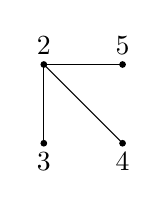
\begin{tikzpicture}
		\draw[black, thin] (0, 1) -- (1, 1);
		\draw[black, thin] (0, 0) -- (0, 1);
		\draw[black, thin] (0, 1) -- (1, 0);
		\filldraw[black] (1,0) circle (1pt) node[anchor=north] {$4$};
		\filldraw[black] (0,0) circle (1pt) node[anchor=north] {$3$};
		\filldraw[black] (0,1) circle (1pt) node[anchor=south] {$2$};
		\filldraw[black] (1,1) circle (1pt) node[anchor=south] {$5$};
	\end{tikzpicture}
	\end{center}
	\caption{The reduced weight graph $G$ of the weight vector $w = \{1, 1, \epsilon, \epsilon, \epsilon\}$.}
	\label{fig:losev-manin5-reduced-graph}
    \end{figure}
    
    Then in order to construct fan,
    we consider the building set of $1$-connected flats,
    whose definition we can recall from Subsection \ref{subsec:graphic-building-set}.
    From the reduced weight graph above, we see that the flats in the graphs are
    \begin{center}
		\begin{tabular}{ |c|c|c|c|} 
		\hline
 		Rank 1 & $F_1$ & $F_2$ & $F_3$  \\ \hline
 		& 
		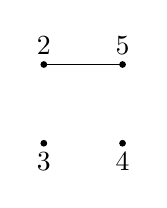
\begin{tikzpicture}
		\draw[black, thin] (0, 1) -- (1, 1);
		\filldraw[black] (1,0) circle (1pt) node[anchor=north] {$4$};
		\filldraw[black] (0,0) circle (1pt) node[anchor=north] {$3$};
		\filldraw[black] (0,1) circle (1pt) node[anchor=south] {$2$};
		\filldraw[black] (1,1) circle (1pt) node[anchor=south] {$5$};
		\end{tikzpicture}
		& 
		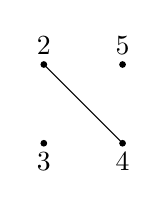
\begin{tikzpicture}
		\draw[black, thin] (0, 1) -- (1, 0);
		\filldraw[black] (1,0) circle (1pt) node[anchor=north] {$4$};
		\filldraw[black] (0,0) circle (1pt) node[anchor=north] {$3$};
		\filldraw[black] (0,1) circle (1pt) node[anchor=south] {$2$};
		\filldraw[black] (1,1) circle (1pt) node[anchor=south] {$5$};
		\end{tikzpicture}
		& 
		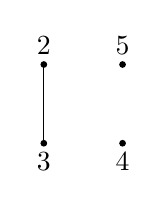
\begin{tikzpicture}
		\draw[black, thin] (0, 1) -- (0, 0);
		\filldraw[black] (1,0) circle (1pt) node[anchor=north] {$4$};
		\filldraw[black] (0,0) circle (1pt) node[anchor=north] {$3$};
		\filldraw[black] (0,1) circle (1pt) node[anchor=south] {$2$};
		\filldraw[black] (1,1) circle (1pt) node[anchor=south] {$5$};
		\end{tikzpicture}
		\\
		\hline
 		Rank 2 & $F_4$ & $F_5$ & $F_6$ \\ \hline
 		& 
		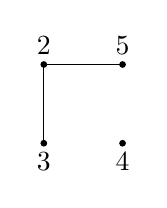
\begin{tikzpicture}
		\draw[black, thin] (0, 1) -- (1, 1);
		\draw[black, thin] (0, 1) -- (0, 0);
		\filldraw[black] (1,0) circle (1pt) node[anchor=north] {$4$};
		\filldraw[black] (0,0) circle (1pt) node[anchor=north] {$3$};
		\filldraw[black] (0,1) circle (1pt) node[anchor=south] {$2$};
		\filldraw[black] (1,1) circle (1pt) node[anchor=south] {$5$};
		\end{tikzpicture}
		& 
		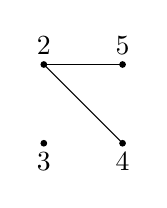
\begin{tikzpicture}
		\draw[black, thin] (0, 1) -- (1, 1);
		\draw[black, thin] (0, 1) -- (1, 0);
		\filldraw[black] (1,0) circle (1pt) node[anchor=north] {$4$};
		\filldraw[black] (0,0) circle (1pt) node[anchor=north] {$3$};
		\filldraw[black] (0,1) circle (1pt) node[anchor=south] {$2$};
		\filldraw[black] (1,1) circle (1pt) node[anchor=south] {$5$};
		\end{tikzpicture}
		& 
		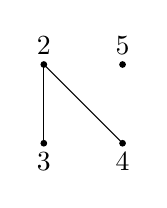
\begin{tikzpicture}
		\draw[black, thin] (0, 1) -- (0, 0);
		\draw[black, thin] (0, 1) -- (1, 0);
		\filldraw[black] (1,0) circle (1pt) node[anchor=north] {$4$};
		\filldraw[black] (0,0) circle (1pt) node[anchor=north] {$3$};
		\filldraw[black] (0,1) circle (1pt) node[anchor=south] {$2$};
		\filldraw[black] (1,1) circle (1pt) node[anchor=south] {$5$};
		\end{tikzpicture}
		\\
		\hline
		\end{tabular}
	\captionof{table}{The $1$-connected flats of $G((1, 1, \epsilon, \epsilon, \epsilon))$.} 
    \end{center}
    Reading off the projection from the graph $G$ as a subgraph of the complete graph on $4$ vertices
    we obtain a list of vectors that give us a combinatorial interpretation of $B'(G)$. 
    The list of projections are obtained as follows:
    \begin{align*}
    \pr_w(v_{1, 2}) = \pr_w(v_{3, 4}) = \pr_w(v_{4, 5}) = \varnothing \\
    \pr_w(v_{1, 3}) = \pr_w(v_{2, 5}) = \pr_w(v_{2, 4}) = V_{F_5} \\
    \pr_w(v_{1, 4}) = \pr_w(v_{2, 5}) = \pr_w(v_{2, 3}) = V_{F_6} \\
    \pr_w(v_{1, 5}) = \pr_w(v_{2, 4}) = \pr_w(v_{2, 3}) = V_{F_4} \\
    \pr_w(v_{2, 3}) = V_{F_3} \\
    \pr_w(v_{2, 4}) = V_{F_2} \\
    \pr_w(v_{2, 5}) = V_{F_1} \\
    \end{align*}
    Since the corresponding flat of each $V_{F_i}$ indicates who the nodes are connected in the phylogenetic trees, 
    by gluing cones defined by phylogenetic trees, 
    we obtain a combinatorial interpretation of the Bergman fan as follows:
    
    \begin{figure}
	\begin{center}
	\begin{tikzpicture}
	    % Draw fan skeleton
		\draw[black, thin] (0, 0) -- (4, 0);
		\draw[black, thin] (0, 0) -- (0, 4);
		\draw[black, thin] (0, 0) -- (0, -4);
		\draw[black, thin] (0, 0) -- (-4, 0);
		\draw[black, thin] (0, 0) -- (4, 4);
		\draw[black, thin] (0, 0) -- (-4, -4);
		\filldraw[black] (4, 0) circle (1pt) node[anchor=south] {$V_{F_5}$};
		\filldraw[black] (4, 4) circle (1pt) node[anchor=south] {$V_{F_1}$};
		\filldraw[black] (0, 4) circle (1pt) node[anchor=south] {$V_{F_4}$};
		\filldraw[black] (0, -4) circle (1pt) node[anchor=north] {$V_{F_2}$};
		\filldraw[black] (-4, -4) circle (1pt) node[anchor=north] {$V_{F_6}$};
		\filldraw[black] (-4, 0) circle (1pt) node[anchor=south] {$V_{F_3}$};
		
		
		% Draw labelled trees 
		% First quadrant
		% Lower
 		\draw (2.6, 2) node[above]{ \tiny 1}-- (4.2, 2) node[above]{\tiny 2};
		\draw (3.0, 2)-- (3.0, 1) node[below]{\tiny 3};
 		\draw (3.4, 2)-- (3.4, 1) node[below]{\tiny 4};
 		\draw (3.8, 2)-- (3.8, 1) node[below]{\tiny 5};

		% Upper
		 \draw (1.0, 4) node[above]{ \tiny 1}-- (2.6, 4) node[above]{\tiny 2};
		\draw (1.4, 4)-- (1.4, 3) node[below]{\tiny 5};
 		\draw (1.8, 4)-- (1.8, 3) node[below]{\tiny 3};
 		\draw (2.2, 4)-- (2.2, 3) node[below]{\tiny 4};
		
		% Second quadrant
		% Lower
		 \draw (-3.4, 2.6) node[above]{ \tiny 1}-- (-1.8, 2.6) node[above]{\tiny 2};
		\draw (-2.2, 2.6)-- (-2.2, 1.6) node[below]{\tiny 3};
 		\draw (-2.6, 2.6)-- (-2.6, 1.6) node[below]{\tiny 5};
 		\draw (-3.0, 2.6)-- (-3.0, 1.6) node[below]{\tiny 4};
		
		% Third quadrant
		% Lower
		\draw (-2.4, -3.0) node[above]{ \tiny 1}-- (-0.8, -3.0) node[above]{\tiny 2};
		\draw (-1.2, -3.0)-- (-1.2, -4.0) node[below]{\tiny 3};
 		\draw (-1.6, -3.0)-- (-1.6, -4.0) node[below]{\tiny 4};
 		\draw (-2.0, -3.0)-- (-2.0, -4.0) node[below]{\tiny 5};
		
		% Upper
		\draw (-4.2, -1.0) node[above]{ \tiny 1}-- (-2.6, -1.0) node[above]{\tiny 2};
		\draw (-3.0, -1.0)-- (-3.0, -2.0) node[below]{\tiny 4};
 		\draw (-3.4, -1.0)-- (-3.4, -2.0) node[below]{\tiny 3};
 		\draw (-3.8, -1.0)-- (-3.8, -2.0) node[below]{\tiny 5};
		
		% Fourth quadrant
		% Lower
		\draw (1.4, -2.0) node[above]{ \tiny 1}-- (3.0, -2.0) node[above]{\tiny 2};
		\draw (2.6, -2.0)-- (2.6, -3.0) node[below]{\tiny 4};
 		\draw (2.2, -2.0)-- (2.2, -3.0) node[below]{\tiny 5};
 		\draw (1.8, -2.0)-- (1.8, -3.0) node[below]{\tiny 3};
		
	\end{tikzpicture}
	\end{center}
	\caption{The combinatorial description of the Bergman fan,
	with each $2$-dimensional cone corresponding to a combinatorial type of the phylogenetic tree -- a type of curve.
	The primitive generators of the one dimensional cones of the fan are $V_{F_{i}}$ for $i \in [6]$. 
	They are vectors $(1, 0), (1, 1), (0,1), (-1, 0), (-1, -1), (0, -1)$ 
	on a plane.}
    \end{figure}
    
    To calculate the cohomology ring of the $\overline{M}_{0, 5}$,
    we first define lattice of flats, which is defined as following:
    \begin{definition}[Lattice of flats]
        A poset of closed subsets of a matroid.    
    \end{definition}
    
    In this example, the building set $\mathcal{G}$ is the set of all flats.
    Then Chow ring $A^\ast(X_{\Sigma_G})$ is the quotient of $\Z[x_\sigma: \sigma \in \mathcal{G}]$ 
    mod out the ideal $SR(\Sigma_\mathcal{G}) + L_{\Sigma_{\mathcal{G}}}$
    where $SR(\Sigma_\mathcal{G})$ is a set of products of rays $v_{F_i}$ that do not form a cone. 
    To calculate the Chow ring, which is equivalent to the cohomology ring in this case, 
    we have 
    \begin{align*}
    	A^\ast(X_{\Sigma_\mathcal{G}}) &= \frac{\Z[x_1, x_2, x_3, x_4, x_5, x_6]}{I_1}\\
	&\cong \frac{\Z[x, y, z, w]}{\langle x^3, y^3, z^3, w^3, x^2 + y^2, x^2 + z^2, x^2 + w^2, xy, xz, xw \rangle}.
    \end{align*}
    where $I = \langle x_1x_2, x_1x_3, x_1x_4, x_2x_3, x_2x_6, x_3x_5, x_4x_5, x_5x_6, x_4x_6, x_1 + x_5 - x_3 - x_4, x_1 + x_6 - x_2 - x_4, x_3 + x_6 - x_2 - x_5 \rangle$.
    The mod-out ideal $I$ can be calculated by calculating 
    the two equivalence relations in previous chapter on Chow ring as follows.
    \begin{enumerate}
    \item[(1)]
	Notice that $V_{F_1}$ can only forms cones with $V_{F_4}$ and $V_{F_5}$;
	$V_{F_2}$ only forms cones with $V_{F_5}$ and $V_{F_6}$;
	$V_{F_3}$ only forms cones with $V_{F_4}$ and $V_{F_6}$;
	$V_{F_4}$ only forms cones with $V_{F_1}$ and $V_{F_3}$;
	$V_{F_5}$ only forms cones with $V_{F_1}$ and $V_{F_2}$;
	$V_{F_6}$ only forms cones with $V_{F_2}$ and $V_{F_3}$.
	We thus set the complimentary product of set of $D_i$'s to zero,
	obtaining
	\begin{align*}
		D_1 D_2 &= D_1 D_3 = D_1 D_6 = 0 \\
		D_2 D_1 &= D_2 D_3 = D_2 D_4 = 0 \\
		D_3 D_1 &= D_3 D_2 = D_3 D_5 = 0 \\
		D_4 D_2 &= D_4 D_5 = D_4 D_6 = 0 \\
		D_5 D_3 &= D_5 D_4 = D_5 D_6 = 0 \\
		D_6 D_1 &= D_6 D_4 = D_6 D_5 = 0 \\
	\end{align*}
	Deleting repetitive information because of commutativity,
	we have 
	\begin{align*}
		D_1 D_2 &= 0 \\
		D_1 D_3 &= 0 \\
		D_1 D_6 &= 0 \\
		D_2 D_3 &= 0 \\
		D_2 D_4 &= 0 \\
		D_3 D_5 &= 0 \\
		D_4 D_5 &= 0 \\
		D_4 D_6 &= 0 \\
		D_5 D_6 &= 0 
 	\end{align*}
	Then pick a basis of this ambient $2$-dimensional 
	ambient vector space $\calb = \{V_{F_4}, V_{F_5}\}$.
	
	\item[(2)]
	For the second relationship,
	we take the sum of inner products of every generators with 
	each element in the basis as follows.
	For $V_{F_4}$ we have
	\[
		\sum\limits_{i=1}^6 \inner{V_{F_i}, V_{F_4}} D_i = 
		D_1 + D_4 - D_2 - D_6 = 0.
	\]
	For $V_{F_5}$ we have
	\[
		\sum\limits_{i=1}^6 \inner{V_{F_i}, V_{F_5}} D_i = 
		D_1 + D_5 - D_3 - D_6 = 0.
	\]
	These two equations give us
	\[
	D_1 + D_5 = D_3 + D_6, D_1 + D_4 = D_2 + D_6
	\]
    \end{enumerate}
    Using these two relations, renaming and canceling out some variables, 
    we obtain the desired cohomology of the Losiv-Manin space. 
    Other Losiv-Manin spaces with $l \ge 3$ will generate similar star-like Bergman combinatorial structures as well,
    for which we can calculate the toric variety and the Chow ring accordingly. 
    
    

%%% Chapter 6: Future Work
\chapter{Future Work}
In this thesis, we survey the theory and methods of computing of cohomology ring of Hassett spaces using techniques of geometric tropicalization, theory of matroids and toric varieties. We gave combinatorial description of the tropicalization of Hassett spaces with weighted vectors that only have $2$ heavy weights (Losev-Manin space) and investigated in depth the calculation of the cohomology of the space.  

For ongoing and future work, we are generalizing the computation of the Chow ring to Hassett spaces with weight vectors that contain more than $2$ heavy weights. 
Increasing the number of heavy weights enlarges drastically the space of phylogenetic trees that parametrizes the combinatorial types, which describes more details and yields delicate combinatorial structures. 
Along this line, we are working on weight vector that contains only $3$ weight vectors and giving detailed combinatorial description of the Bergman. 

%%% Appendix 
\appendix
\include{appendix}

\include{source_code}

\backmatter

\bibliographystyle{hmcmath} 

\bibliography{mybib}

\end{document}
